\documentclass[aspectratio=169,12pt,handout]{beamer}
\usepackage{pgfpages}
\pgfpagesuselayout{resize to}[letterpaper,landscape,border shrink=5mm]
\usetheme{Madrid}
\usecolortheme{default}
\usepackage{graphicx}
\usepackage{booktabs}
\usepackage{amsmath}

% Clean colors
\definecolor{binggreen}{RGB}{0,100,0}
\setbeamercolor{structure}{fg=binggreen}
\setbeamercolor{title}{fg=white,bg=binggreen}
\setbeamercolor{frametitle}{fg=white,bg=binggreen}

\setbeamertemplate{navigation symbols}{}
\setbeamertemplate{footline}[frame number]

\hypersetup{pdfpagelayout=SinglePage}

\title{Gene Expression Pattern Matching}
\subtitle{Evaluating Similarity Metrics for NMF Constraint Patterns}
\author{}
\institute{Binghamton University}
\date{April 2026}

\begin{document}

% ------------------------------------------------------------------
\begin{frame}
\titlepage
\end{frame}

% ------------------------------------------------------------------
\begin{frame}{Motivation}
\begin{itemize}
  \item \textbf{Goal:} Identify genes whose expression over time matches
        biologically observed constraint patterns
  \item \textbf{Data:} $\sim$17,856 genes across 4 timepoints (0, 3, 6, 9)
        in 4 clusters, raw and log-transformed
  \item \textbf{Problem with NMF:} All factors are non-negative, so NMF
        ranks genes by coefficient magnitude, not shape match.
        Up-regulation and down-regulation are conflated.
  \item \textbf{Our approach:} Compare 6 similarity metrics that directly
        measure gene--pattern shape similarity
\end{itemize}
\end{frame}

% ------------------------------------------------------------------
\begin{frame}{Constraint Patterns}
\begin{center}
\begin{tabular}{lccccl}
\toprule
\textbf{Cluster} & \textbf{t=0} & \textbf{t=3} & \textbf{t=6} & \textbf{t=9} & \textbf{Shape} \\
\midrule
One   & 1.45  & 12.0  & 5.21  & 6.51  & Spike at t=3 \\
Two   & 0.371 & 0.803 & 1.22  & 1.78  & Steady increase \\
Three & 0.041 & 0.0   & 0.037 & 0.035 & Near-flat, dip at t=3 \\
Four  & 0.009 & 0.638 & 0.018 & 0.024 & 70$\times$ spike at t=3 \\
\bottomrule
\end{tabular}
\end{center}

\vspace{0.5em}
\small
All data min-max normalized to $(0, 1]$ before comparison.
Both raw and log-transformed (LT) versions analyzed.
\end{frame}

% ------------------------------------------------------------------
\begin{frame}{The 6 Metrics at a Glance}
\begin{center}
\small
\begin{tabular}{llll}
\toprule
\textbf{Metric} & \textbf{Measures} & \textbf{Ranking} & \textbf{Key property} \\
\midrule
Pearson  & Shape (mean-centered) & Higher = better & Scale \& shift invariant \\
Cosine   & Vector angle (raw)    & Higher = better & No mean-centering \\
DTW      & Time-aligned distance & Lower = better  & Allows temporal warping \\
Fr\'{e}chet & Max curve deviation   & Lower = better  & Worst-point sensitive \\
MSE      & Avg squared error     & Lower = better  & Simplest distance \\
sMAPE    & Symmetric \% error    & Lower = better  & Relative scale \\
\bottomrule
\end{tabular}
\end{center}
\end{frame}

% ==================================================================
% RESULTS — clusterOne LT
% ==================================================================
\begin{frame}{Results: clusterOne LT --- Modest Consensus}
\begin{columns}[T]
\begin{column}{0.45\textwidth}
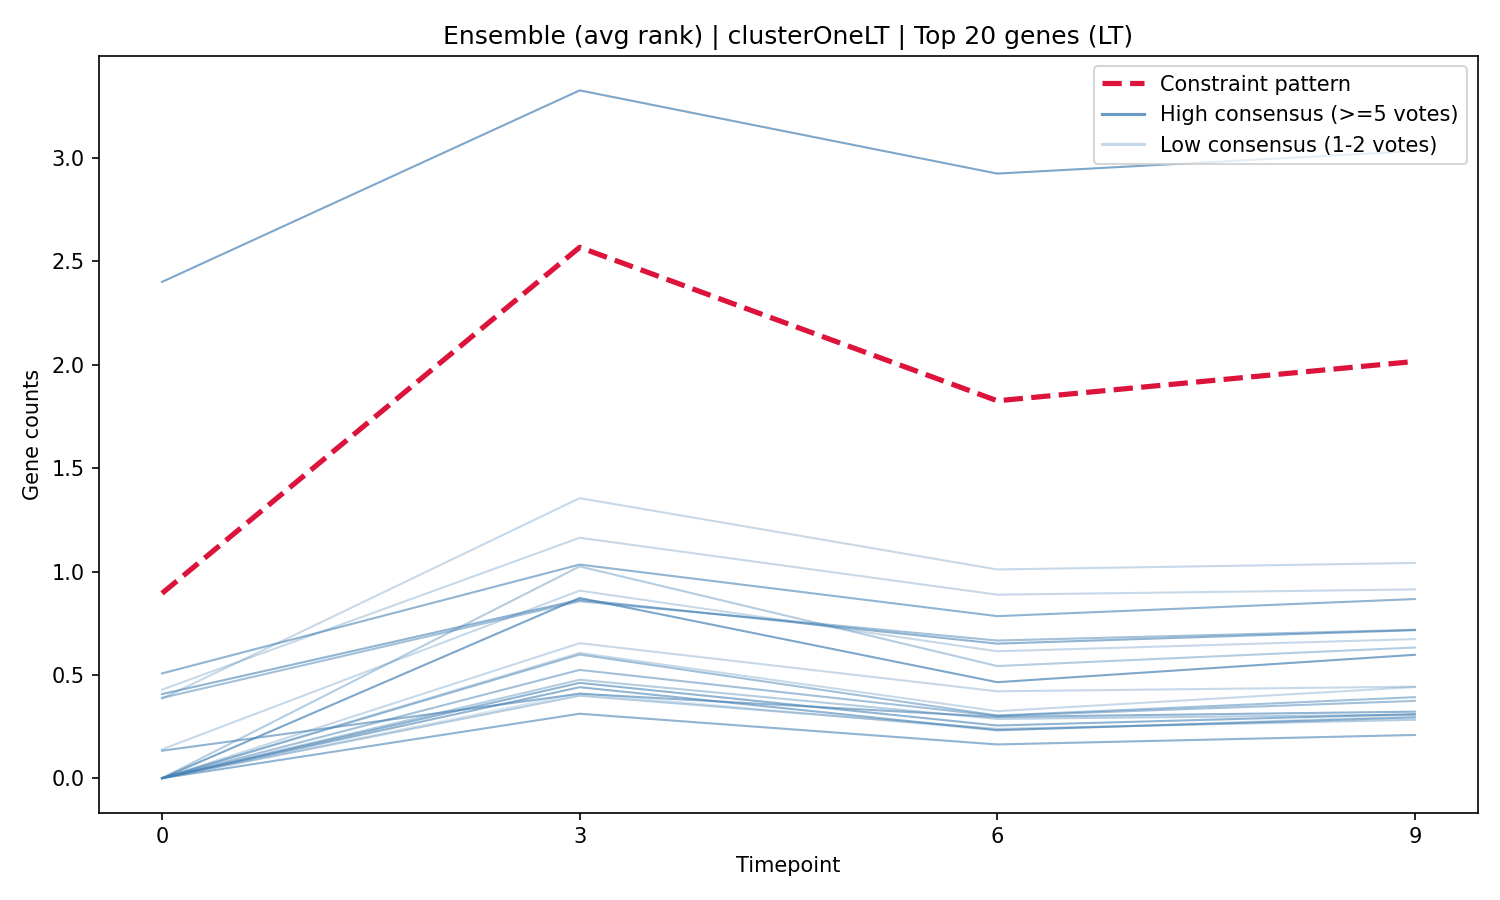
\includegraphics[width=\textwidth]{plots/Ensemble_LT_clusterOneLT_constraint.png}
\end{column}
\begin{column}{0.52\textwidth}
\small
\textbf{2 genes} achieve 5/6 votes:\\[0.3em]
NACA, AC008875.3\\[0.5em]
4 additional genes at 4/6:\\
CCDC57, RTRAF, MDFIC, CTDSPL2\\[0.5em]
Spike-at-$t=3$ pattern --- distance/correlation
methods converge, but no unanimous calls.
\end{column}
\end{columns}
\end{frame}

% ------------------------------------------------------------------
\begin{frame}{Results: clusterOne LT --- Pearson/Fr\'{e}chet/MSE Core}
\begin{columns}[T]
\begin{column}{0.45\textwidth}
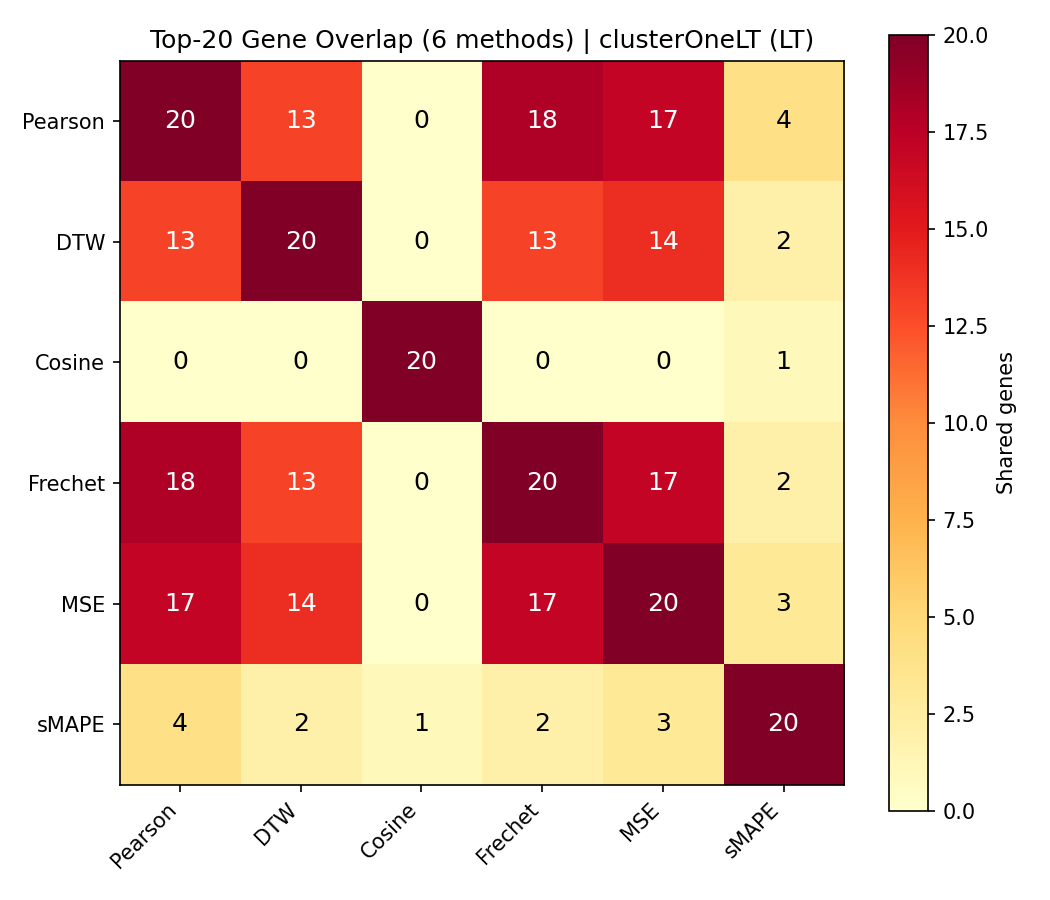
\includegraphics[width=\textwidth]{plots/overlap_6methods_LT_clusterOneLT.png}
\end{column}
\begin{column}{0.52\textwidth}
\small
Pearson--Fr\'{e}chet--MSE: 17--18/20 overlap\\
DTW joins at 13--14/20\\
Cosine isolated: 0/20\\
sMAPE isolated: 1--4/20\\[0.5em]
Cosine fails even on log-transformed\\
data --- magnitude bias persists.\\[0.5em]
sMAPE penalizes relative error\\
on near-zero values.
\end{column}
\end{columns}
\end{frame}

% ------------------------------------------------------------------
\begin{frame}{Ensemble Rankings --- clusterOne (LT)}
\small
\begin{center}
\begin{tabular}{clcl}
\toprule
\textbf{Rank} & \textbf{Gene} & \textbf{Votes} & \textbf{Methods} \\
\midrule
1 & NACA       & \textbf{5/6} & Pearson, DTW, Fr\'{e}chet, MSE, sMAPE \\
2 & AC008875.3 & \textbf{5/6} & Pearson, DTW, Fr\'{e}chet, MSE, sMAPE \\
3 & CCDC57     & 4/6 & Pearson, DTW, Fr\'{e}chet, MSE \\
4 & RTRAF      & 4/6 & Pearson, DTW, Fr\'{e}chet, MSE \\
5 & MDFIC      & 4/6 & Pearson, DTW, Fr\'{e}chet, MSE \\
\bottomrule
\end{tabular}
\end{center}

\vspace{0.5em}
NACA and AC008875.3 are the highest-confidence candidates for the
clusterOne LT spike pattern --- consistent across 5 of 6 methods.
\end{frame}

% ==================================================================
% RESULTS — clusterTwo LT
% ==================================================================
\begin{frame}{Results: clusterTwo LT --- Best Agreement}
\begin{columns}[T]
\begin{column}{0.45\textwidth}
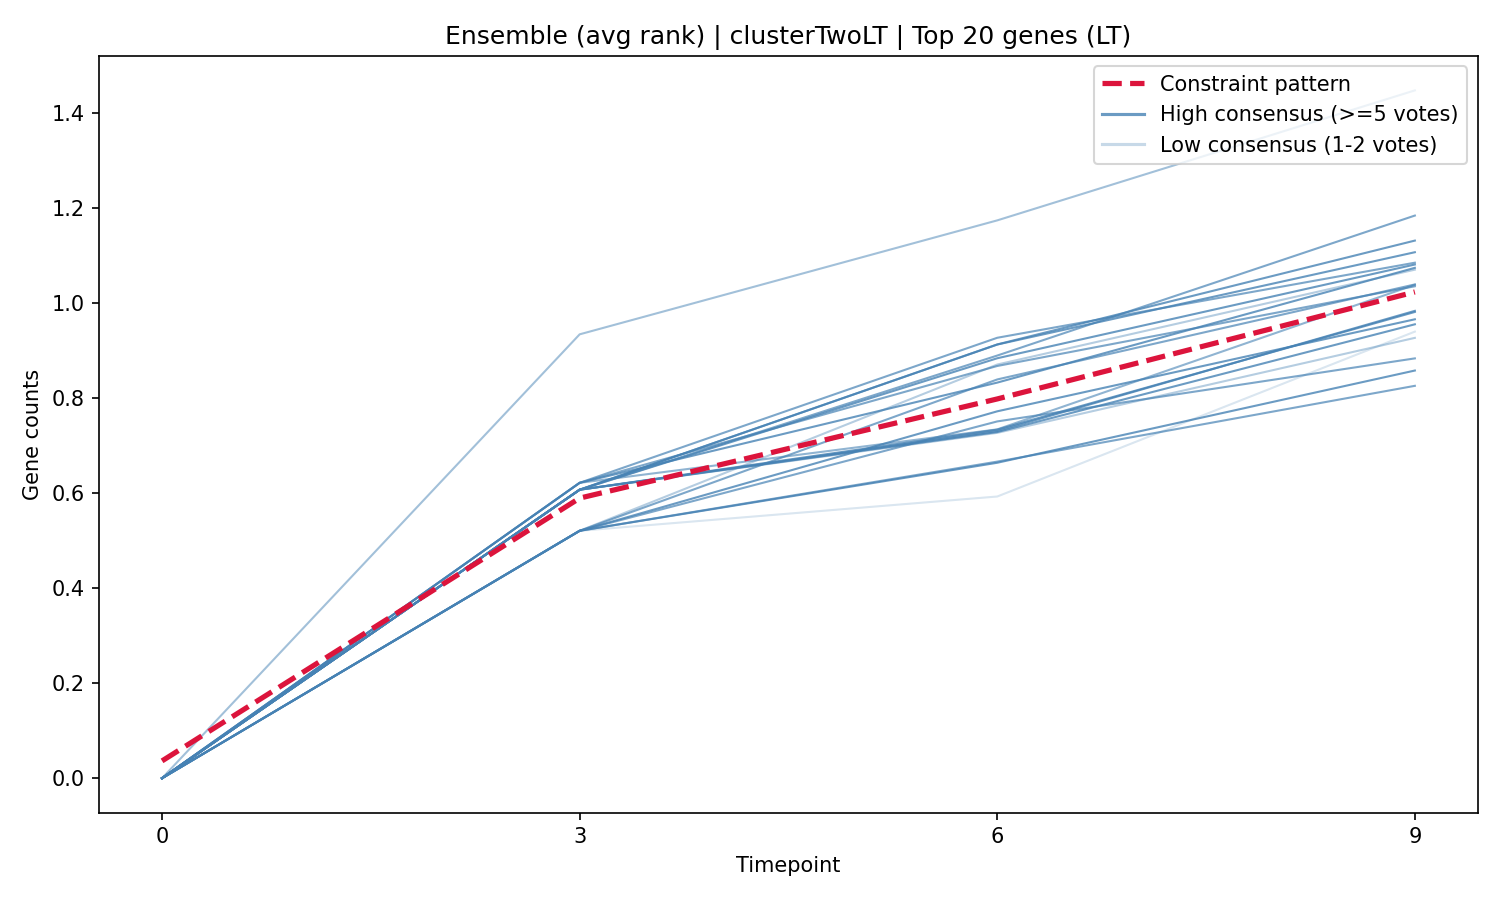
\includegraphics[width=\textwidth]{plots/Ensemble_LT_clusterTwoLT_constraint.png}
\end{column}
\begin{column}{0.52\textwidth}
\small
\textbf{9 of top 11 genes} achieve unanimous 6/6 votes:\\[0.3em]
RAB14, SYNGR1, ARHGAP25,\\
HNRNPH3, BSG, CAPN2,\\
NOL7, ZC3H15, PRDX6\\[0.5em]
Steady-increase pattern is easiest
to match --- all methods converge.\\[0.5em]
\textbf{Highest-confidence candidates}\\for biological follow-up.
\end{column}
\end{columns}
\end{frame}

% ------------------------------------------------------------------
\begin{frame}{Results: clusterTwo LT --- All Methods Converge}
\begin{columns}[T]
\begin{column}{0.45\textwidth}
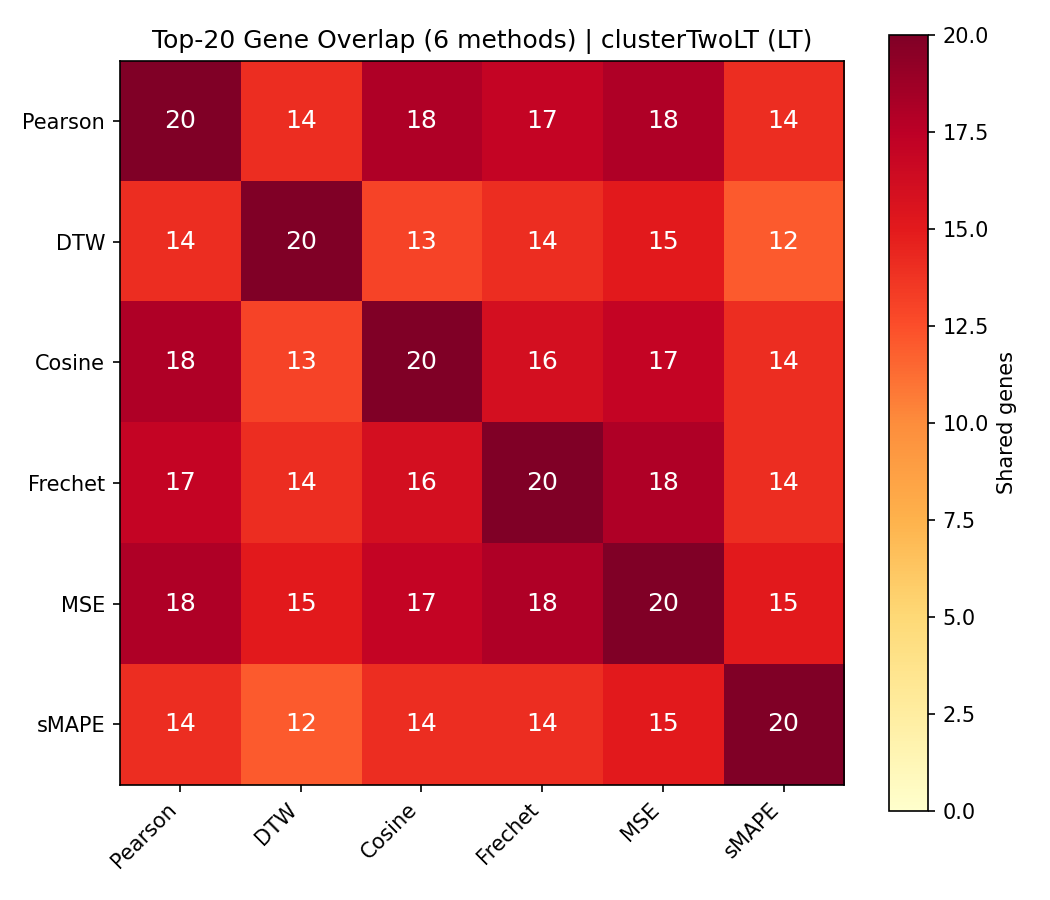
\includegraphics[width=\textwidth]{plots/overlap_6methods_LT_clusterTwoLT.png}
\end{column}
\begin{column}{0.52\textwidth}
\small
\textbf{Most balanced cluster overall.}\\[0.3em]
Pearson--MSE: 18/20\\
Pearson--Cosine: 18/20\\
Fr\'{e}chet--MSE: 18/20\\[0.5em]
Even sMAPE agrees: 12--15/20\\
across all methods --- no zero-value failure here.\\[0.5em]
Steady-increase pattern is robust\\
across all 6 metrics.
\end{column}
\end{columns}
\end{frame}

% ------------------------------------------------------------------
\begin{frame}{Ensemble Rankings --- clusterTwo (LT)}
\small
\begin{center}
\begin{tabular}{clcl}
\toprule
\textbf{Rank} & \textbf{Gene} & \textbf{Votes} & \textbf{Methods} \\
\midrule
1 & RAB14    & \textbf{6/6} & All methods \\
2 & SYNGR1   & \textbf{6/6} & All methods \\
3 & ARHGAP25 & \textbf{6/6} & All methods \\
4 & HNRNPH3  & \textbf{6/6} & All methods \\
5 & BSG      & \textbf{6/6} & All methods \\
\bottomrule
\end{tabular}
\end{center}

\vspace{0.5em}
9 of the top 11 genes are unanimous 6/6 across all methods ---
highest-confidence candidates for TCR pathway involvement.
\end{frame}

% ==================================================================
% RESULTS — clusterThree LT
% ==================================================================
\begin{frame}{Results: clusterThree LT --- 5 of 6 Methods Agree}
\begin{columns}[T]
\begin{column}{0.45\textwidth}
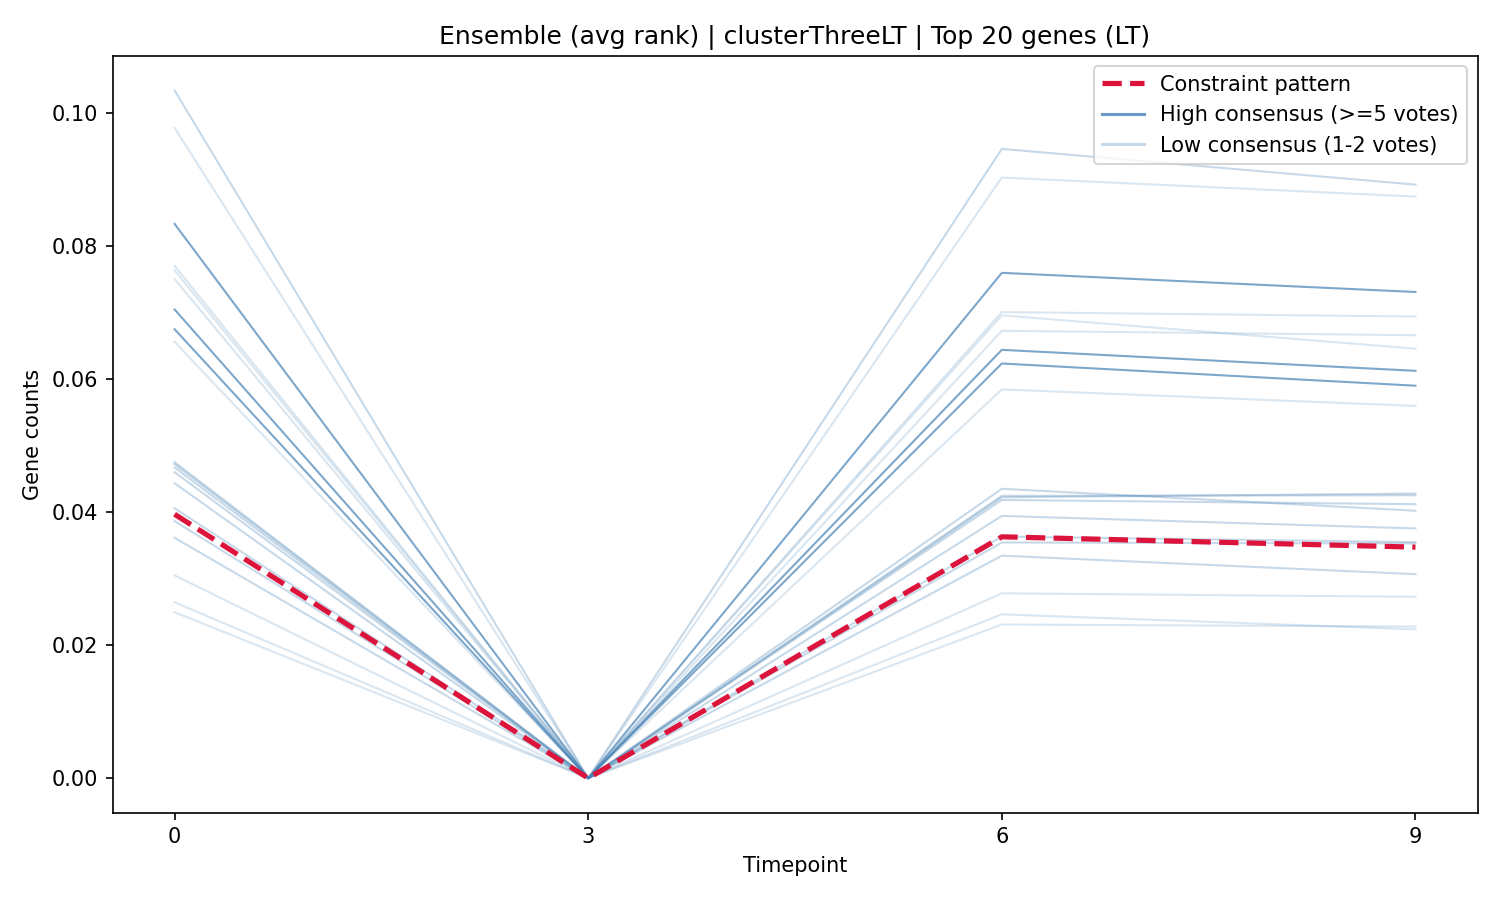
\includegraphics[width=\textwidth]{plots/Ensemble_LT_clusterThreeLT_constraint.png}
\end{column}
\begin{column}{0.52\textwidth}
\small
\textbf{3 genes} achieve 5/6 votes:\\[0.3em]
TEDC1, CTBP1-AS, PGAP1\\[0.5em]
Pearson, DTW, Cosine, Fr\'{e}chet, MSE\\
all converge on the near-flat dip pattern.\\[0.5em]
sMAPE blocked by zero at $t=3$:\\
$\frac{2|0 - g_i|}{|0| + |g_i|} = 2$ regardless of $g_i$.
\end{column}
\end{columns}
\end{frame}

% ------------------------------------------------------------------
\begin{frame}{Results: clusterThree LT --- Strong Consensus (Except sMAPE)}
\begin{columns}[T]
\begin{column}{0.45\textwidth}
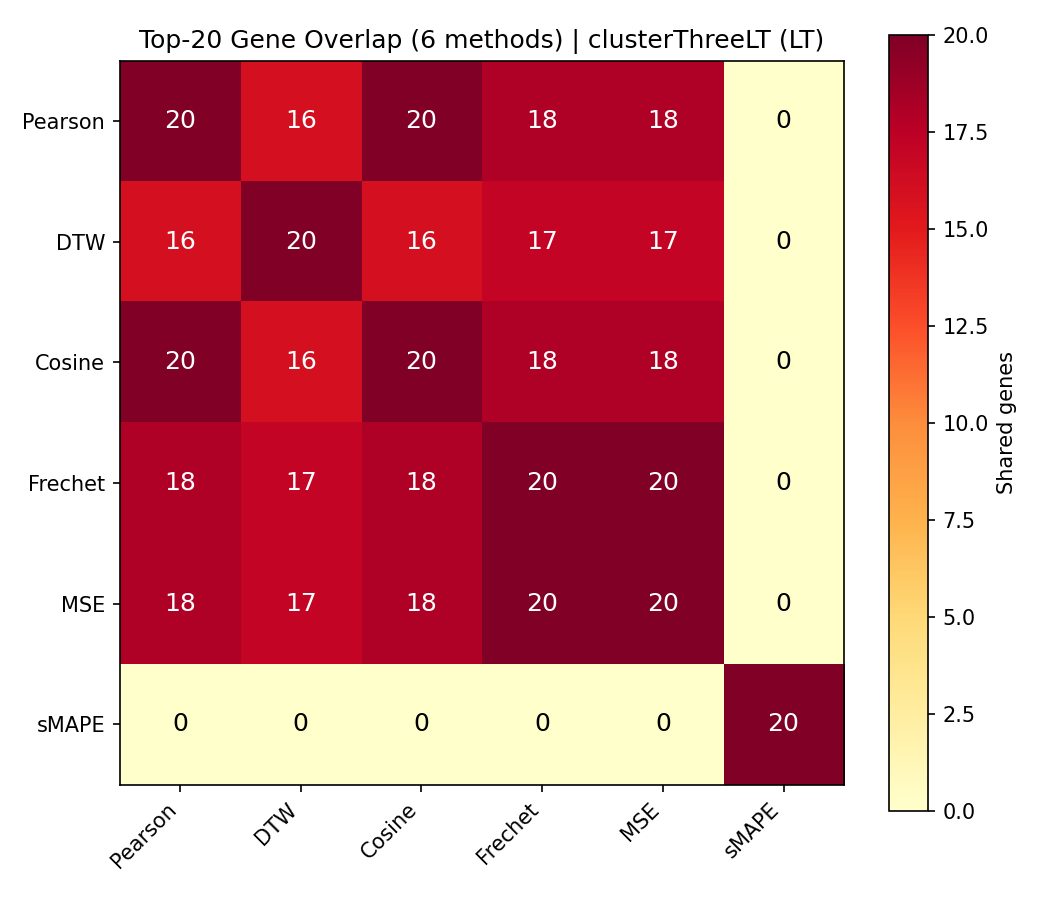
\includegraphics[width=\textwidth]{plots/overlap_6methods_LT_clusterThreeLT.png}
\end{column}
\begin{column}{0.52\textwidth}
\small
Pearson--Cosine: \textbf{20/20} (perfect)\\
Fr\'{e}chet--MSE: \textbf{20/20} (perfect)\\
Cross-pairs: 16--18/20\\[0.5em]
sMAPE: \textbf{0/20} with everything\\
(zero-value failure at $t=3$).\\[0.5em]
\textbf{Validates that 5 of 6 methods\\capture the same biology.}
\end{column}
\end{columns}
\end{frame}

% ------------------------------------------------------------------
\begin{frame}{Ensemble Rankings --- clusterThree (LT)}
\small
\begin{center}
\begin{tabular}{clcl}
\toprule
\textbf{Rank} & \textbf{Gene} & \textbf{Votes} & \textbf{Methods} \\
\midrule
1 & TEDC1    & \textbf{5/6} & Pearson, DTW, Cosine, Fr\'{e}chet, MSE \\
2 & CTBP1-AS & \textbf{5/6} & Pearson, DTW, Cosine, Fr\'{e}chet, MSE \\
3 & PGAP1    & \textbf{5/6} & Pearson, DTW, Cosine, Fr\'{e}chet, MSE \\
\bottomrule
\end{tabular}
\end{center}

\vspace{0.5em}
TEDC1, CTBP1-AS, and PGAP1 are the high-confidence consensus
genes for clusterThree LT (sMAPE excluded due to the zero-at-$t{=}3$ failure).
\end{frame}

% ==================================================================
% RESULTS — clusterFour LT
% ==================================================================
\begin{frame}{Results: clusterFour LT --- The Hard Case}
\begin{columns}[T]
\begin{column}{0.45\textwidth}
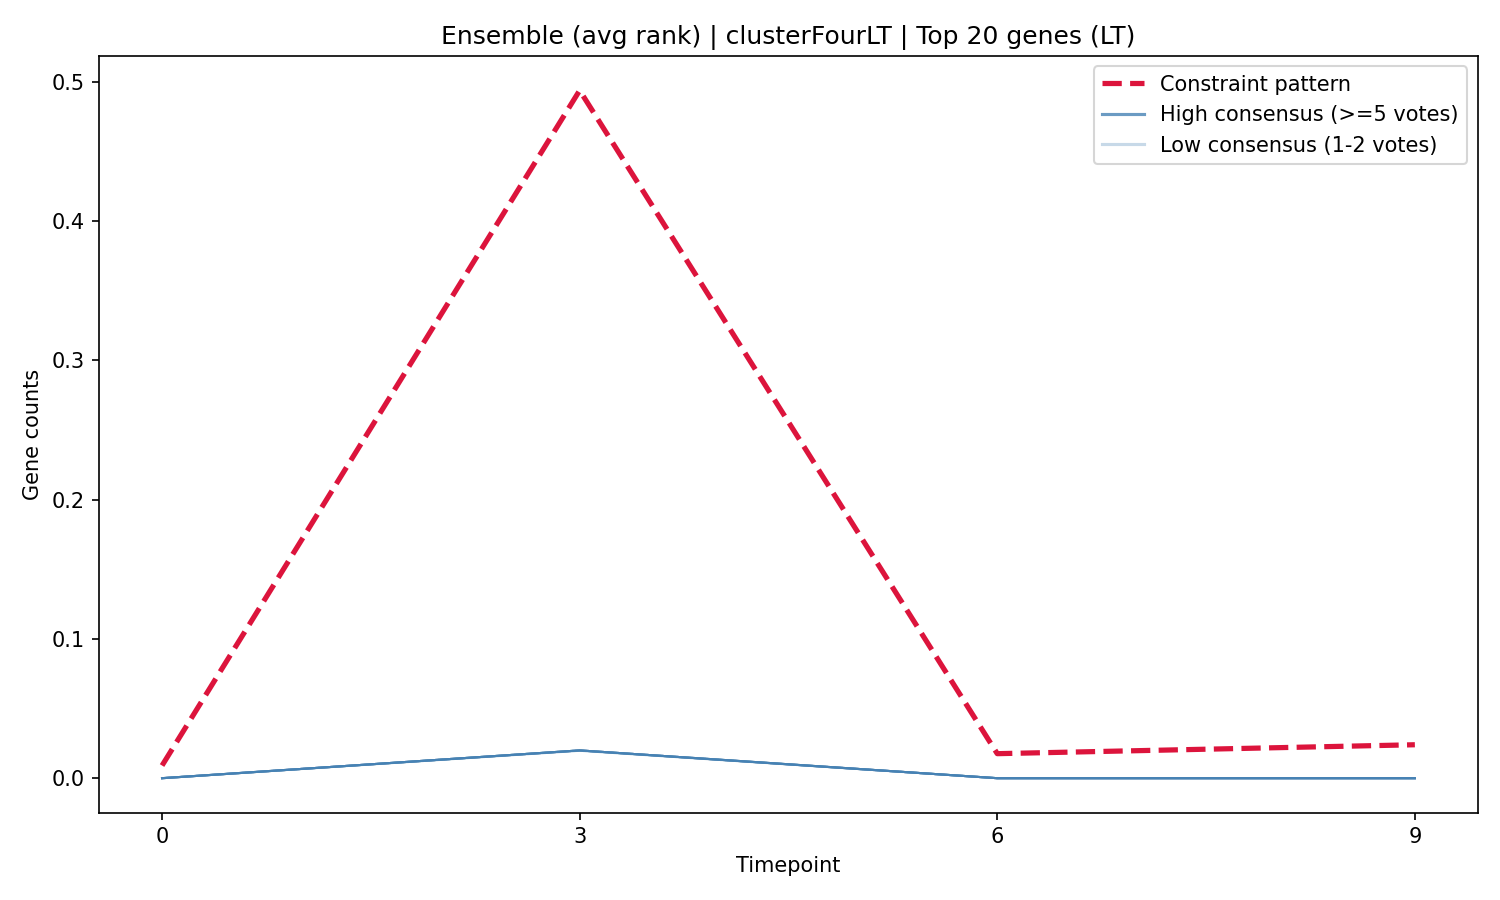
\includegraphics[width=\textwidth]{plots/Ensemble_LT_clusterFourLT_constraint.png}
\end{column}
\begin{column}{0.52\textwidth}
\small
70$\times$ spike at $t=3$ $\Rightarrow$ effectively\\
a delta function.\\[0.5em]
\textbf{Zero genes} achieve $\geq$2/6 votes\\
in the ensemble top-20.\\[0.5em]
Methods split into 3 disjoint groups:
\begin{itemize}\itemsep0pt
\item Cosine/Fr\'{e}chet/MSE (magnitude)
\item Pearson (relative shape)
\item DTW, sMAPE (each isolated)
\end{itemize}
\end{column}
\end{columns}
\end{frame}

% ------------------------------------------------------------------
\begin{frame}{Results: clusterFour LT --- No Shape Consensus}
\begin{columns}[T]
\begin{column}{0.45\textwidth}
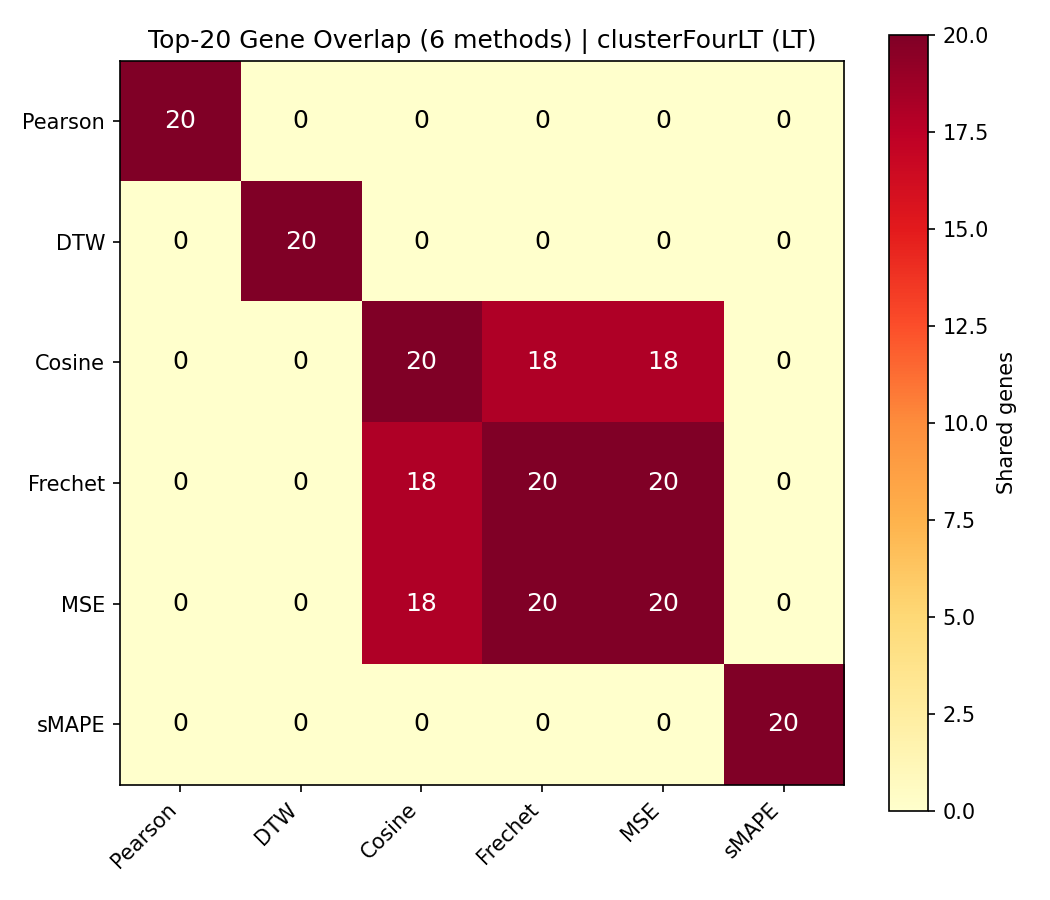
\includegraphics[width=\textwidth]{plots/overlap_6methods_LT_clusterFourLT.png}
\end{column}
\begin{column}{0.52\textwidth}
\small
Cosine--Fr\'{e}chet--MSE: 18--20/20\\
(all dominated by $t=3$ magnitude)\\[0.3em]
Pearson: 0/20 with everything\\
(scale-invariant, finds \textit{relative} peaks)\\[0.3em]
DTW: 0/20 with everything\\
sMAPE: 0/20 with everything\\[0.5em]
\textbf{Needs denser time sampling}\\
to resolve shape vs magnitude.
\end{column}
\end{columns}
\end{frame}

% ------------------------------------------------------------------
\begin{frame}{Ensemble Rankings --- clusterFour (LT)}
\small
\begin{center}
\begin{tabular}{clcl}
\toprule
\textbf{Rank} & \textbf{Gene} & \textbf{Votes} & \textbf{Methods} \\
\midrule
1 & AC068888.2 & 0/6 & --- \\
2 & AC018638.6 & 0/6 & --- \\
3 & SLC16A5    & 0/6 & --- \\
4 & TPH1       & 0/6 & --- \\
5 & CNN3       & 0/6 & --- \\
\bottomrule
\end{tabular}
\end{center}

\vspace{0.5em}
\textbf{No consensus.} Top genes by average rank do not appear in
\textit{any} single method's top-20 --- the 70$\times$ spike defeats the
voting ensemble. clusterFour requires denser temporal sampling.
\end{frame}

% ==================================================================
% APPENDIX: All Methods — LT Clusters
% ==================================================================
\appendix
\begin{frame}{}
\centering
\vfill
{\Huge\textbf{Appendix}}\\[1em]
{\large All Methods — Log-Transformed Clusters}
\vfill
\end{frame}

% --- clusterOne LT ---
\begin{frame}{clusterOne LT — Pearson}
\centering
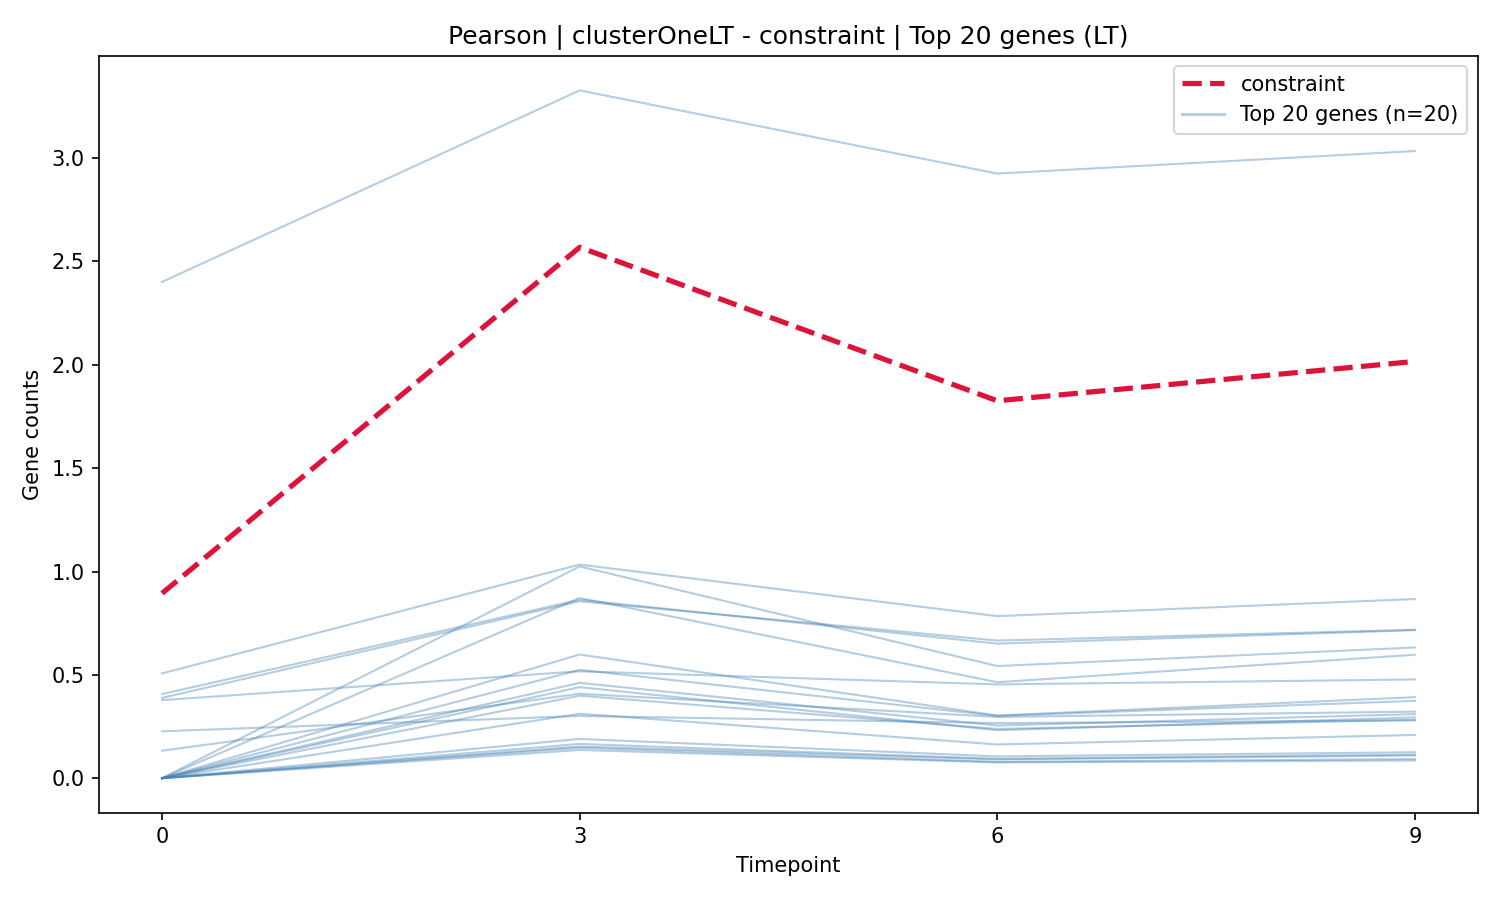
\includegraphics[height=0.85\textheight]{plots/Pearson_LT_clusterOneLT_constraint.png}
\end{frame}

\begin{frame}{clusterOne LT — DTW}
\centering
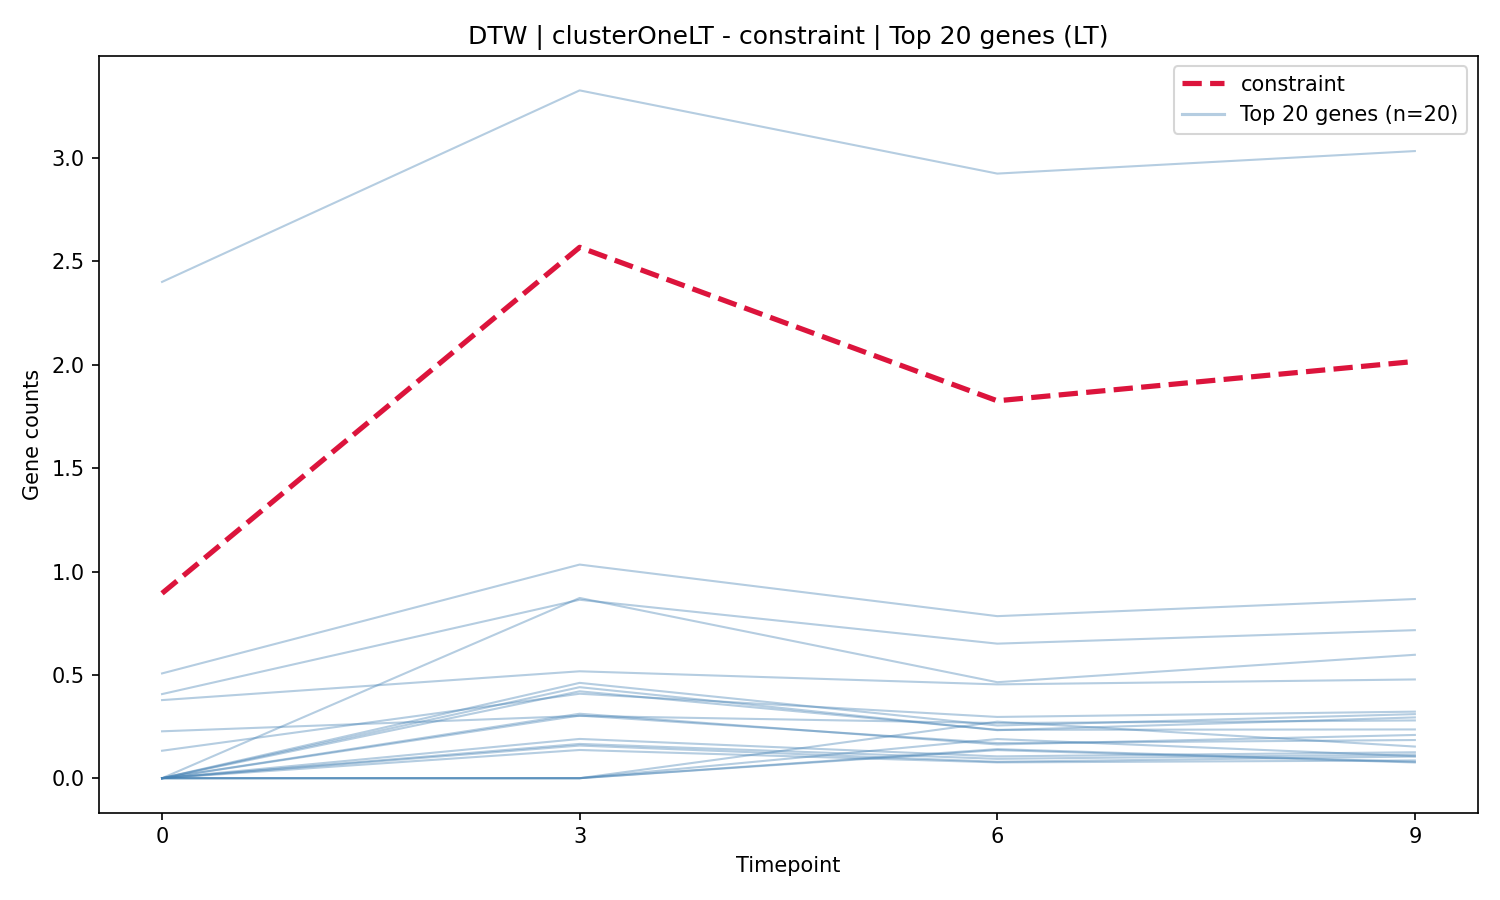
\includegraphics[height=0.85\textheight]{plots/DTW_LT_clusterOneLT_constraint.png}
\end{frame}

\begin{frame}{clusterOne LT — Cosine}
\centering
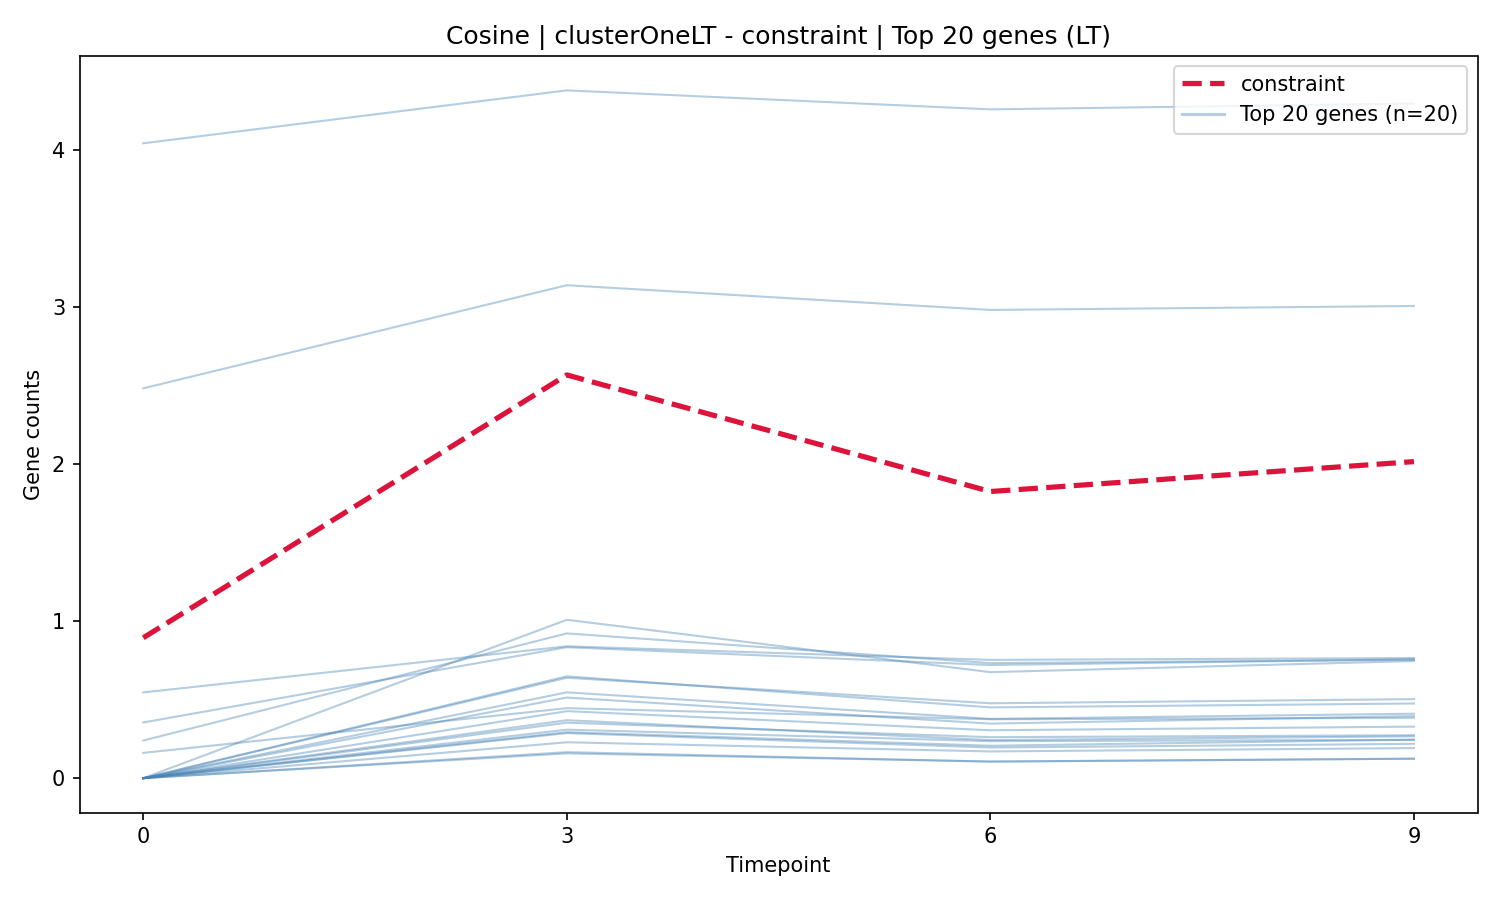
\includegraphics[height=0.85\textheight]{plots/Cosine_LT_clusterOneLT_constraint.png}
\end{frame}

\begin{frame}{clusterOne LT — Fr\'{e}chet}
\centering
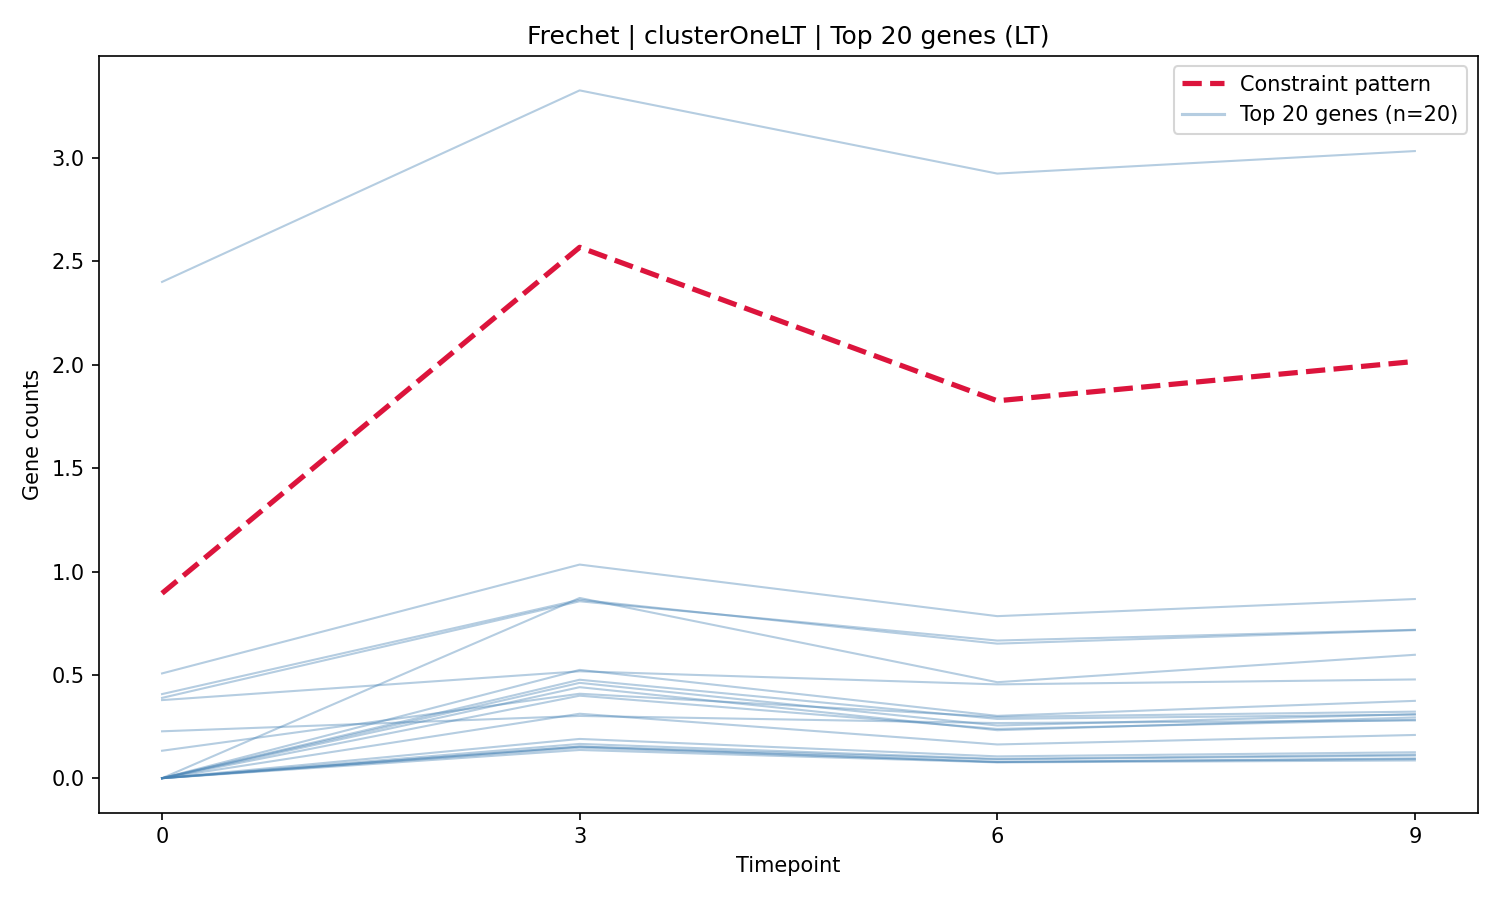
\includegraphics[height=0.85\textheight]{plots/Frechet_LT_clusterOneLT_constraint.png}
\end{frame}

\begin{frame}{clusterOne LT — MSE}
\centering
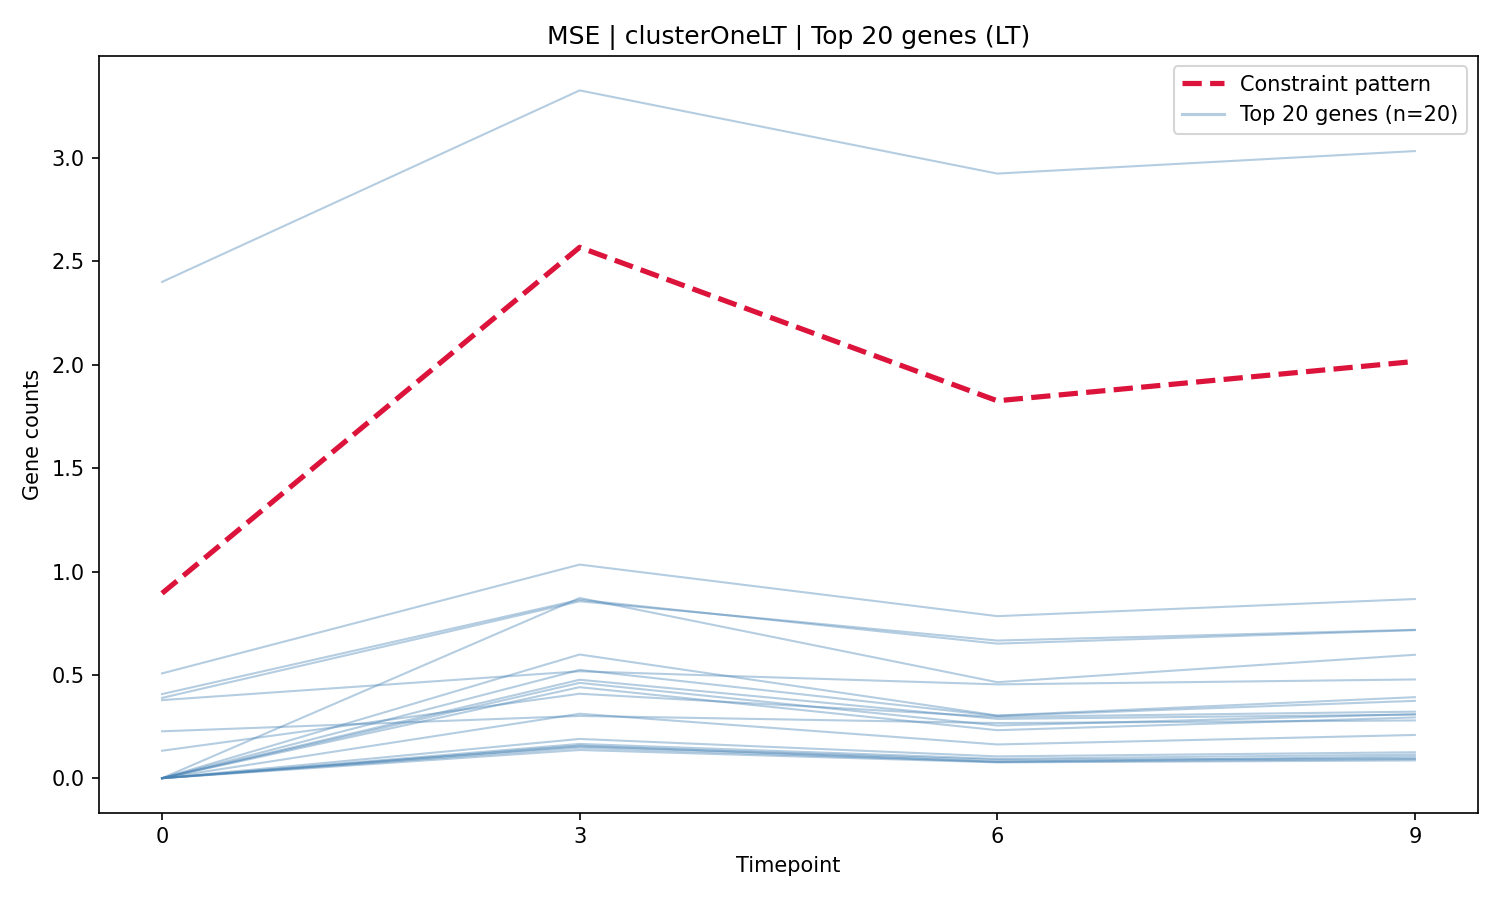
\includegraphics[height=0.85\textheight]{plots/MSE_LT_clusterOneLT_constraint.png}
\end{frame}

\begin{frame}{clusterOne LT — sMAPE}
\centering
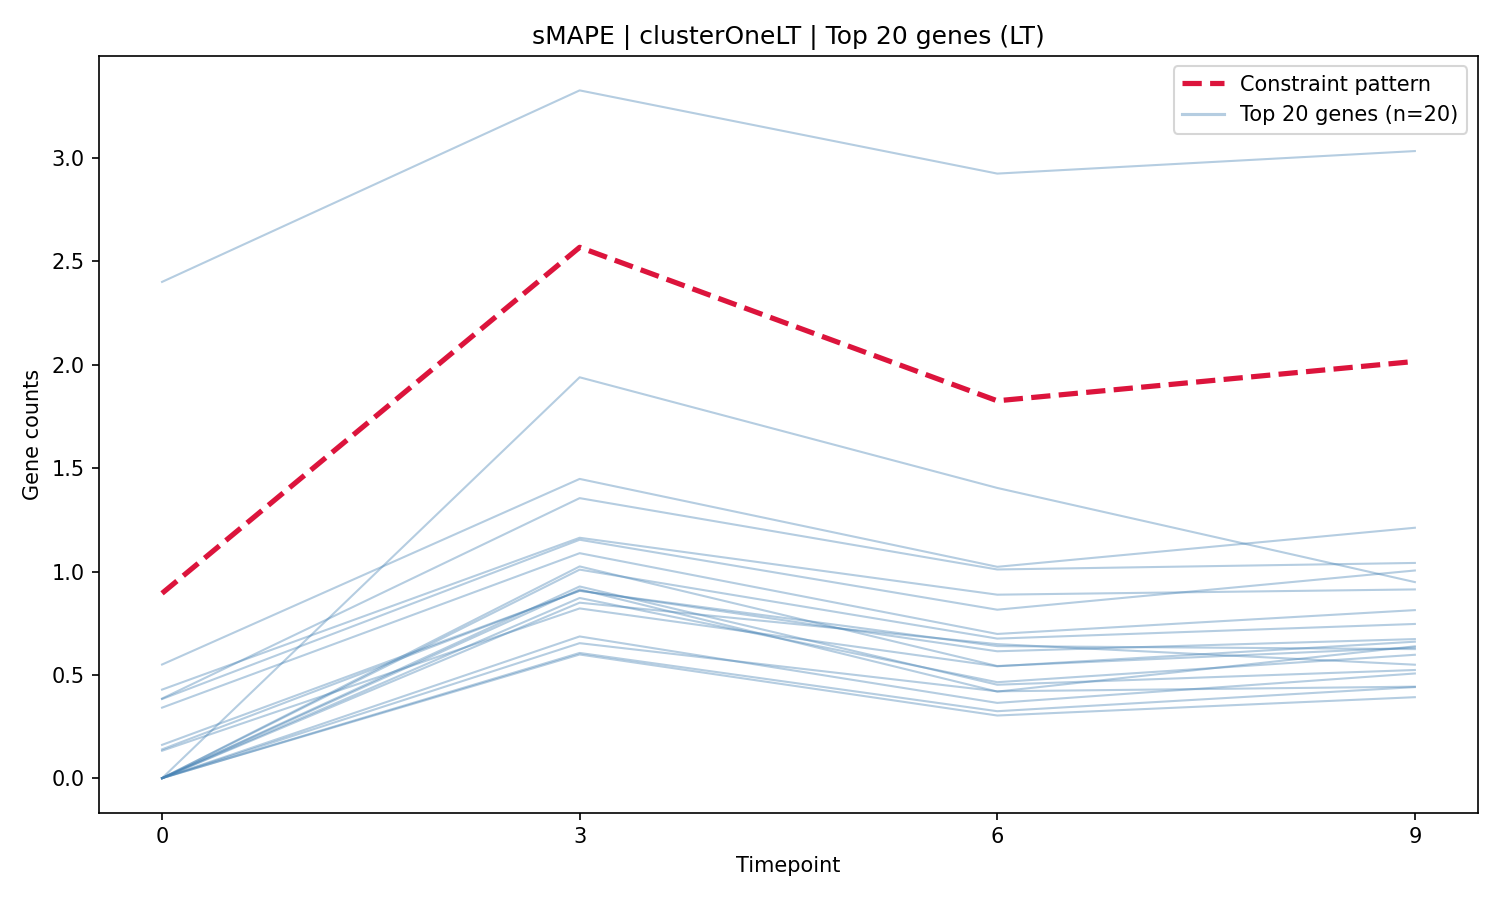
\includegraphics[height=0.85\textheight]{plots/sMAPE_LT_clusterOneLT_constraint.png}
\end{frame}

\begin{frame}{clusterOne LT — Ensemble}
\centering
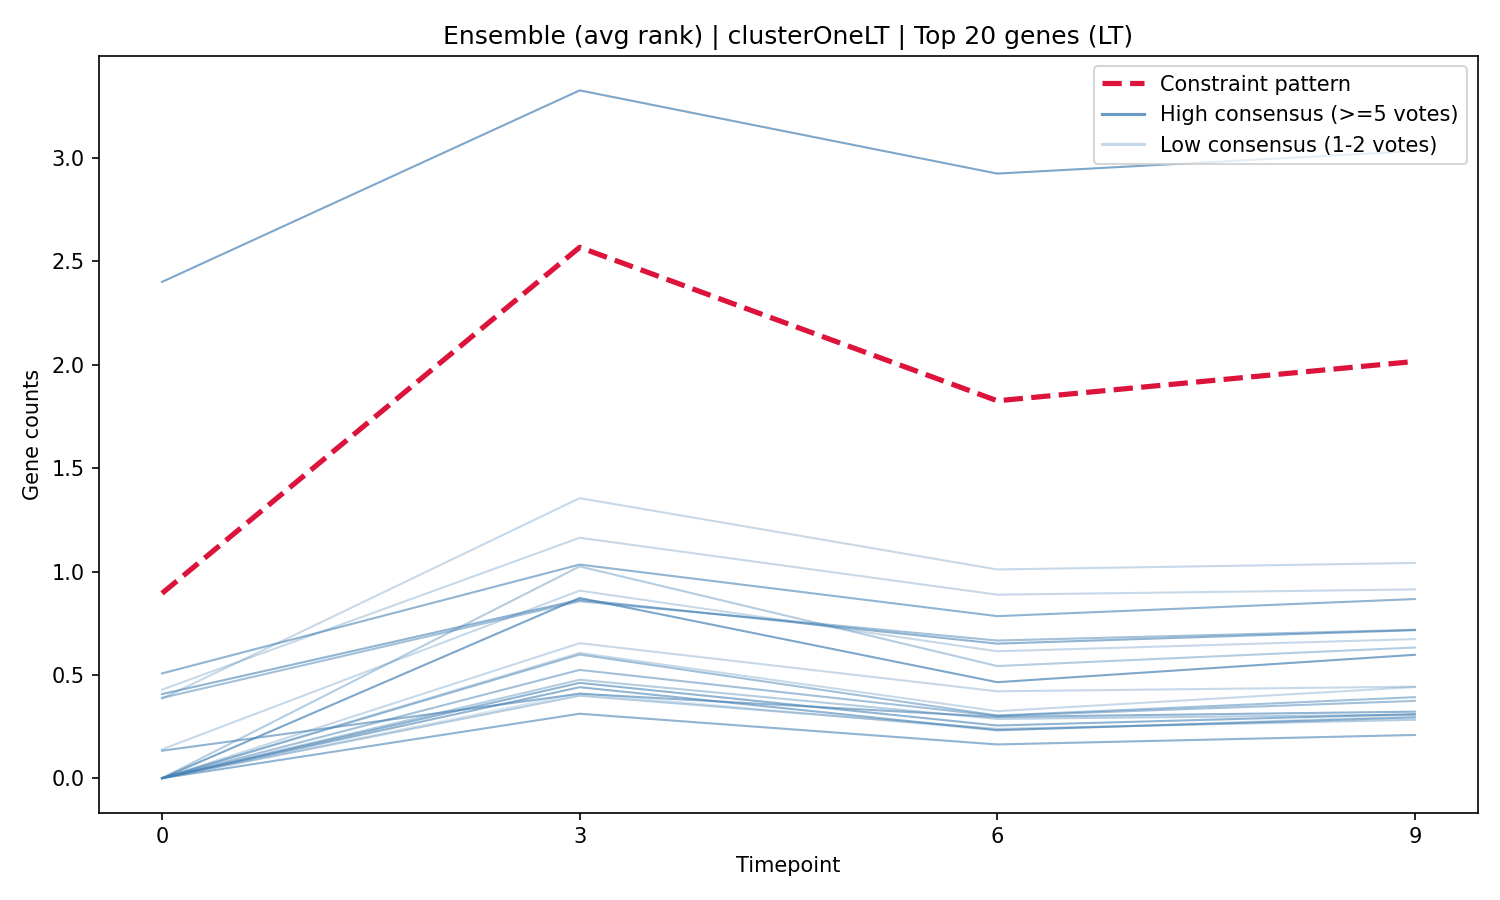
\includegraphics[height=0.85\textheight]{plots/Ensemble_LT_clusterOneLT_constraint.png}
\end{frame}

\begin{frame}{clusterOne LT — Overlap Heatmap}
\centering
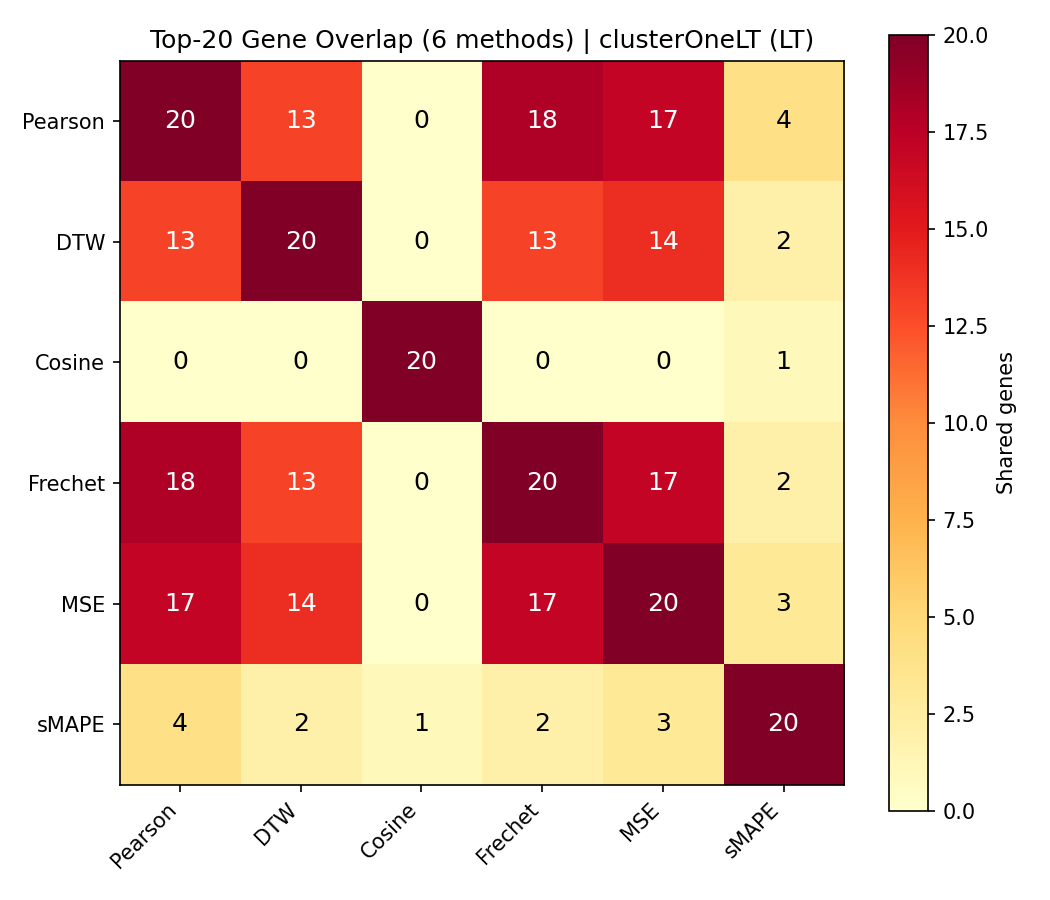
\includegraphics[height=0.85\textheight]{plots/overlap_6methods_LT_clusterOneLT.png}
\end{frame}

% --- clusterTwo LT ---
\begin{frame}{clusterTwo LT — Pearson}
\centering
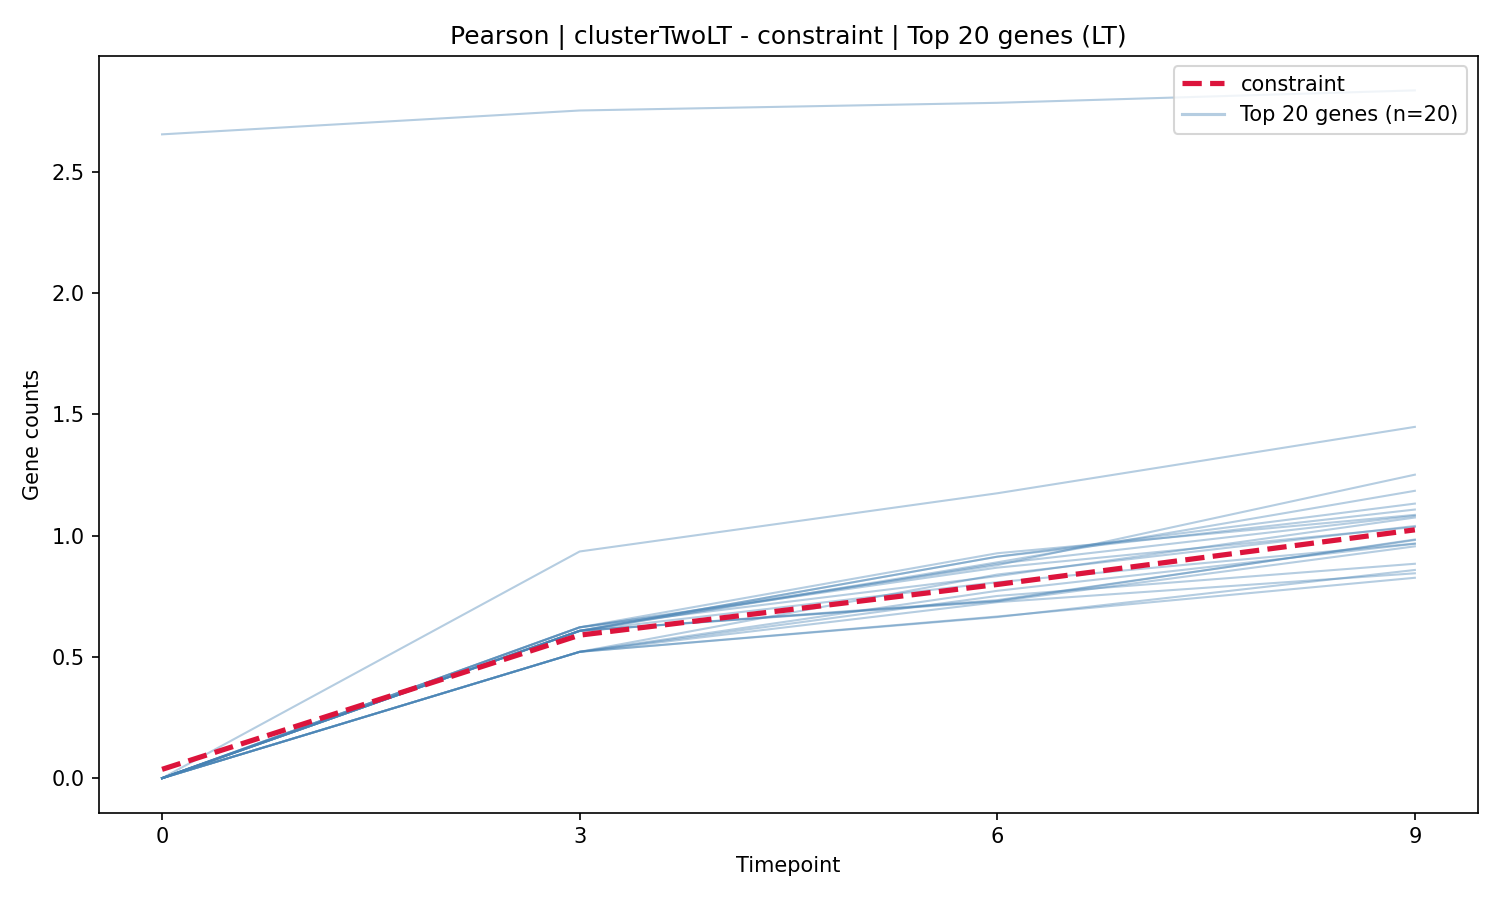
\includegraphics[height=0.85\textheight]{plots/Pearson_LT_clusterTwoLT_constraint.png}
\end{frame}

\begin{frame}{clusterTwo LT — DTW}
\centering
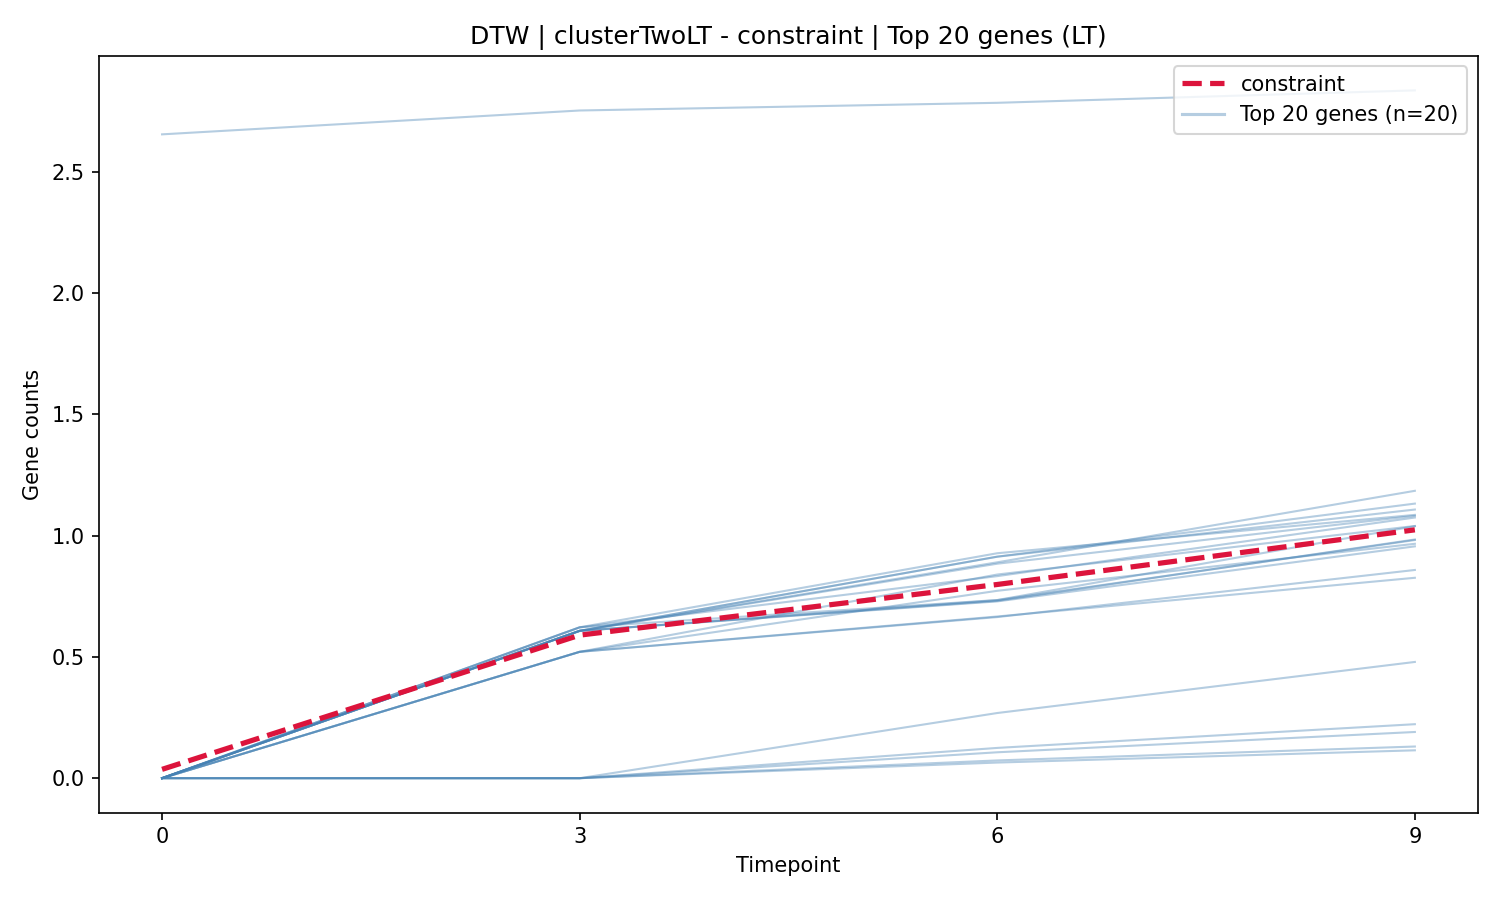
\includegraphics[height=0.85\textheight]{plots/DTW_LT_clusterTwoLT_constraint.png}
\end{frame}

\begin{frame}{clusterTwo LT — Cosine}
\centering
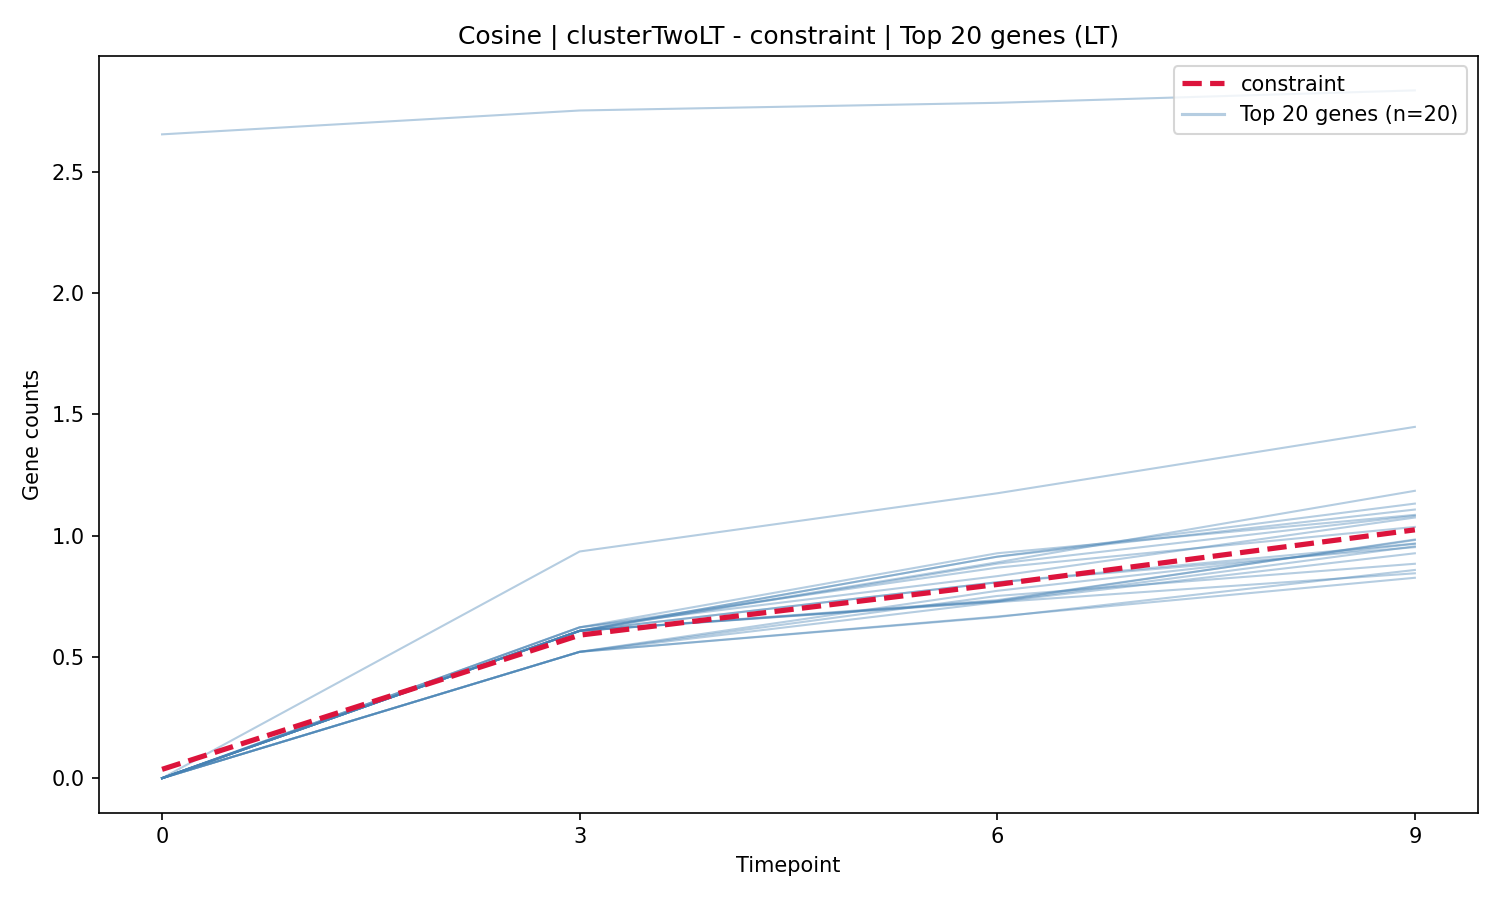
\includegraphics[height=0.85\textheight]{plots/Cosine_LT_clusterTwoLT_constraint.png}
\end{frame}

\begin{frame}{clusterTwo LT — Fr\'{e}chet}
\centering
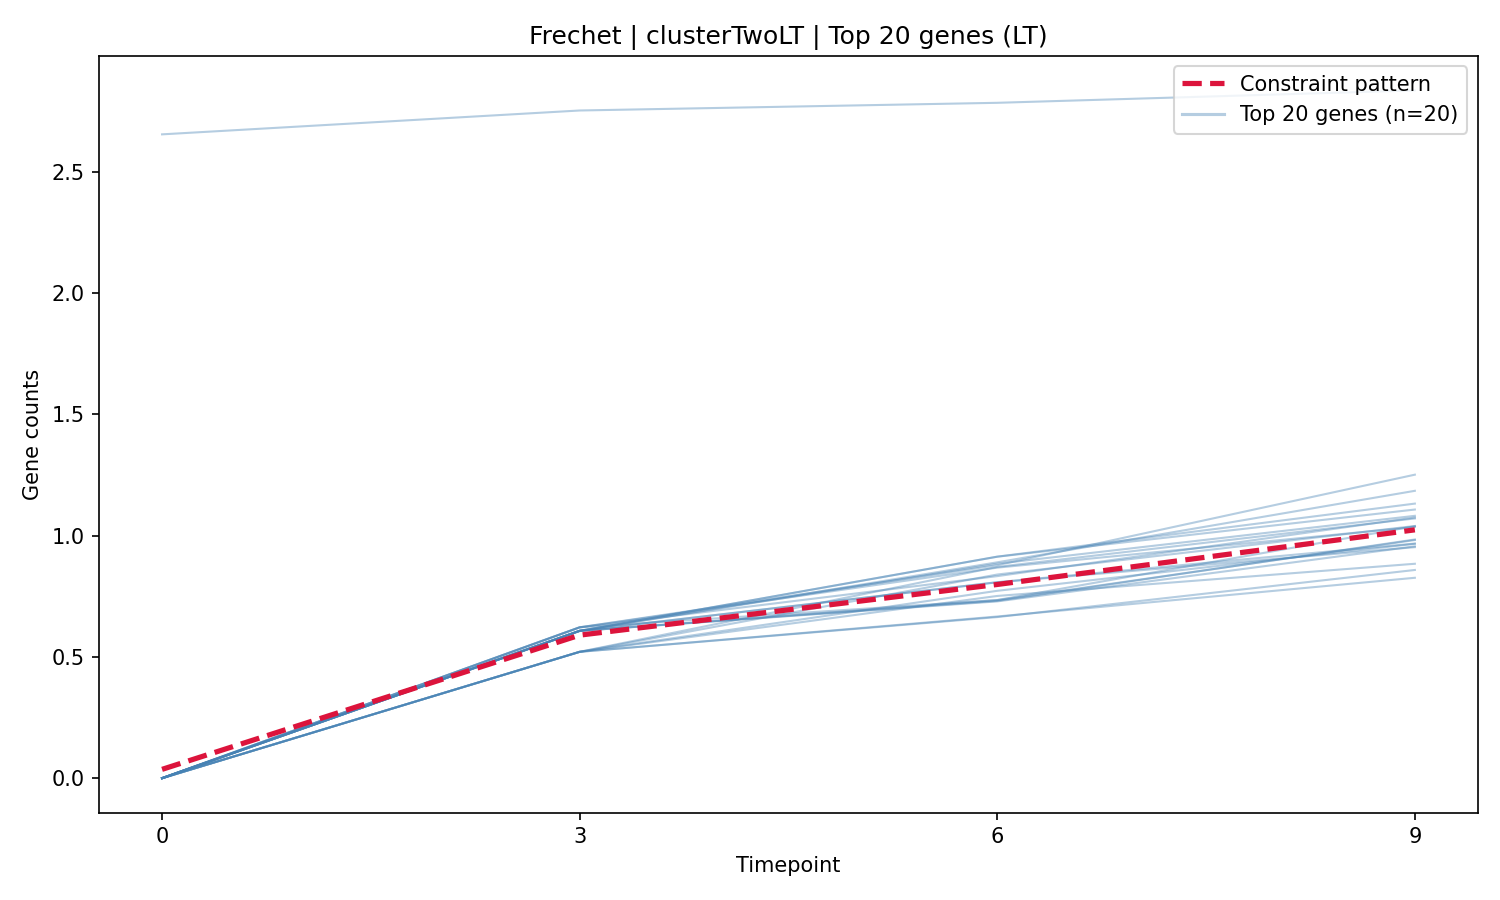
\includegraphics[height=0.85\textheight]{plots/Frechet_LT_clusterTwoLT_constraint.png}
\end{frame}

\begin{frame}{clusterTwo LT — MSE}
\centering
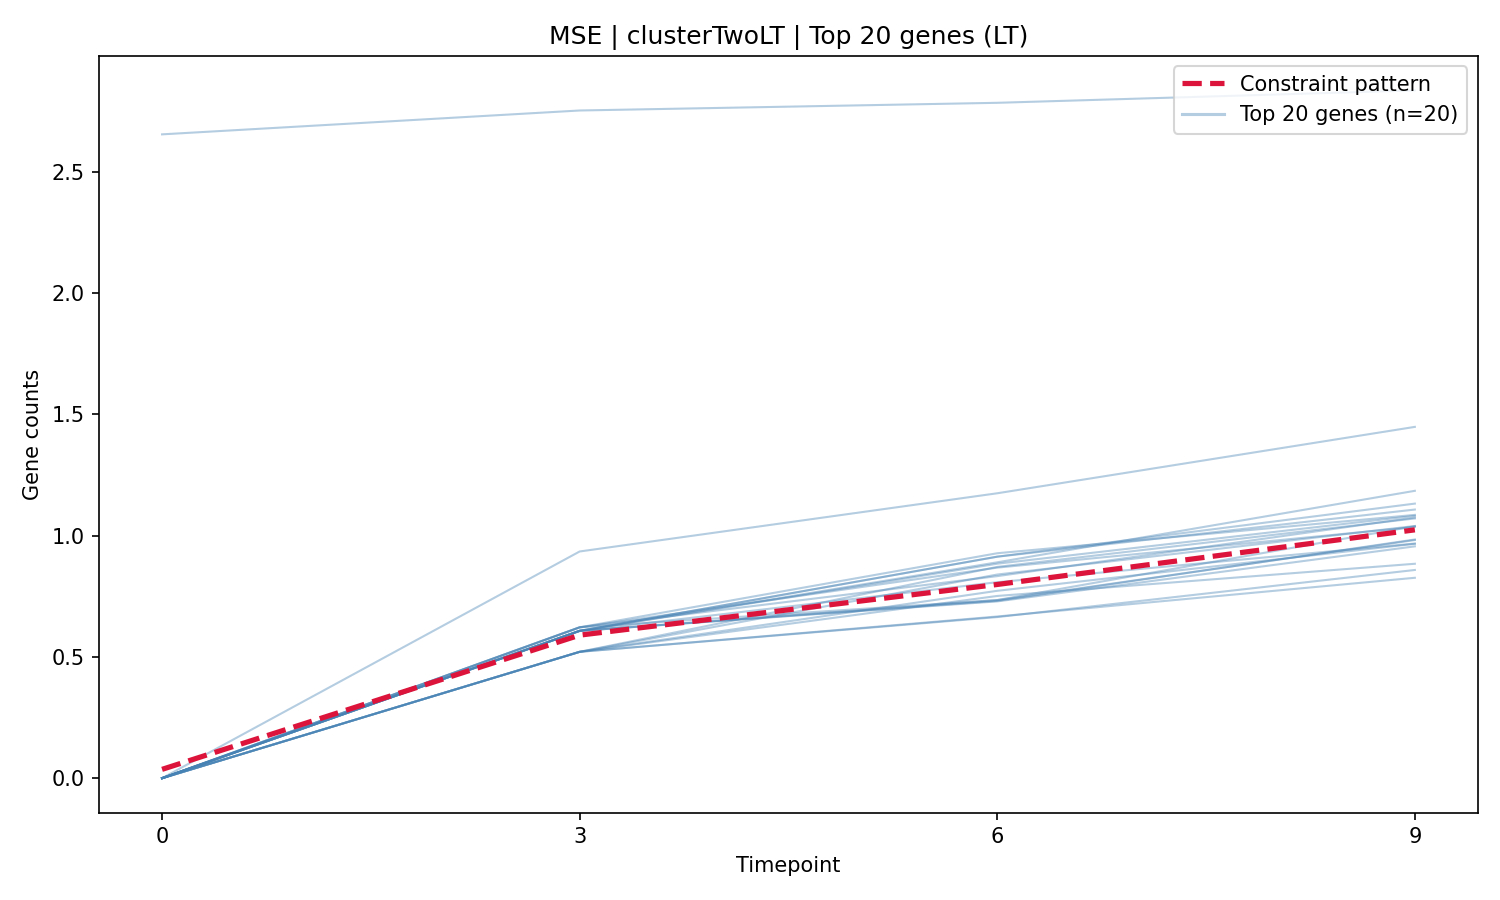
\includegraphics[height=0.85\textheight]{plots/MSE_LT_clusterTwoLT_constraint.png}
\end{frame}

\begin{frame}{clusterTwo LT — sMAPE}
\centering
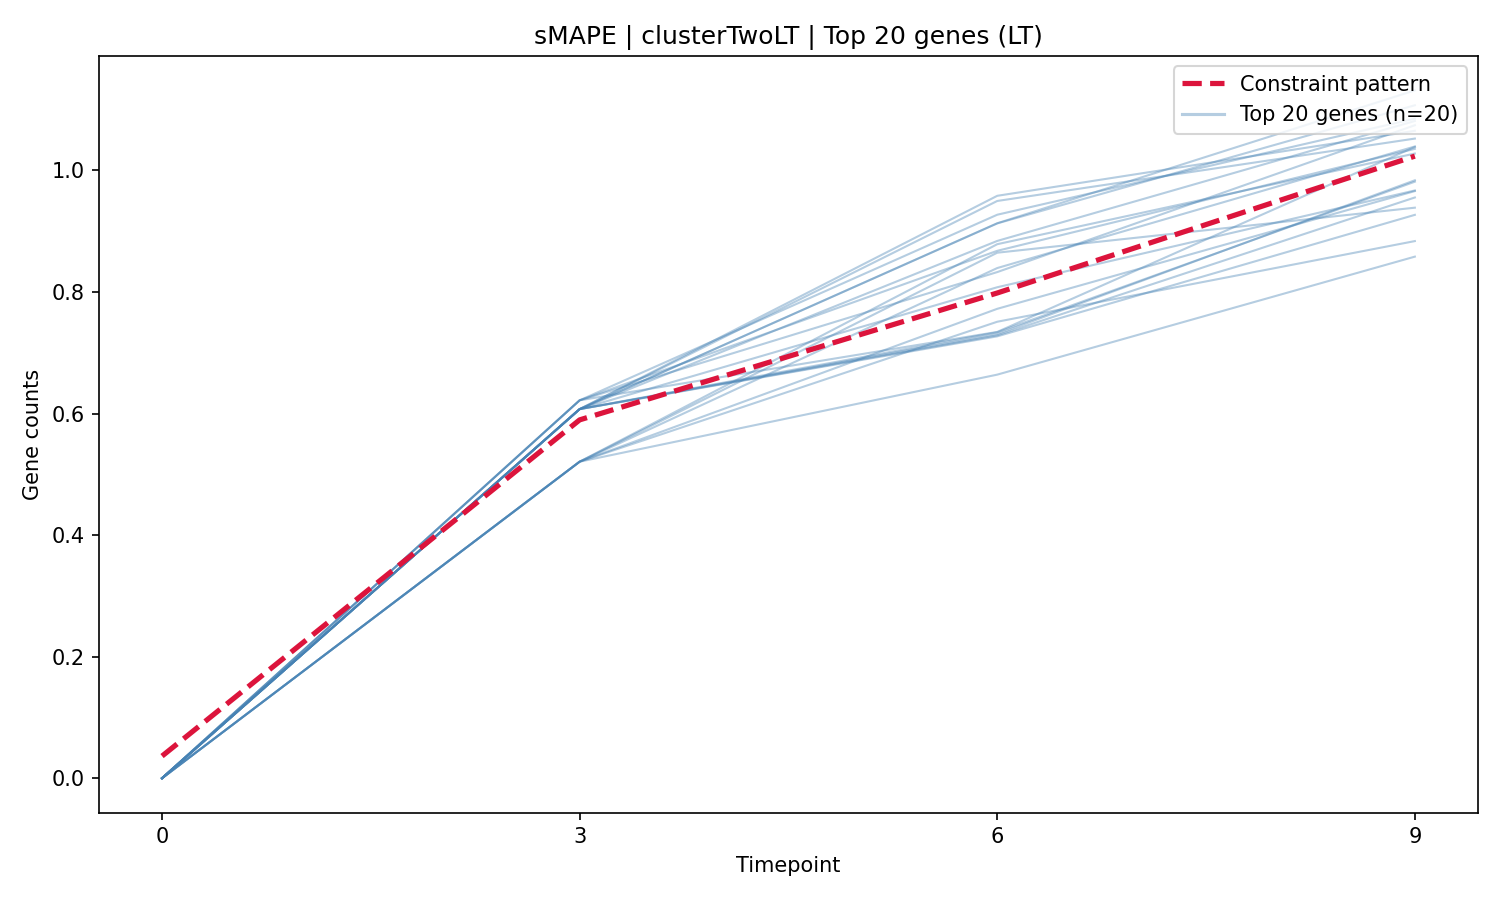
\includegraphics[height=0.85\textheight]{plots/sMAPE_LT_clusterTwoLT_constraint.png}
\end{frame}

\begin{frame}{clusterTwo LT — Ensemble}
\centering
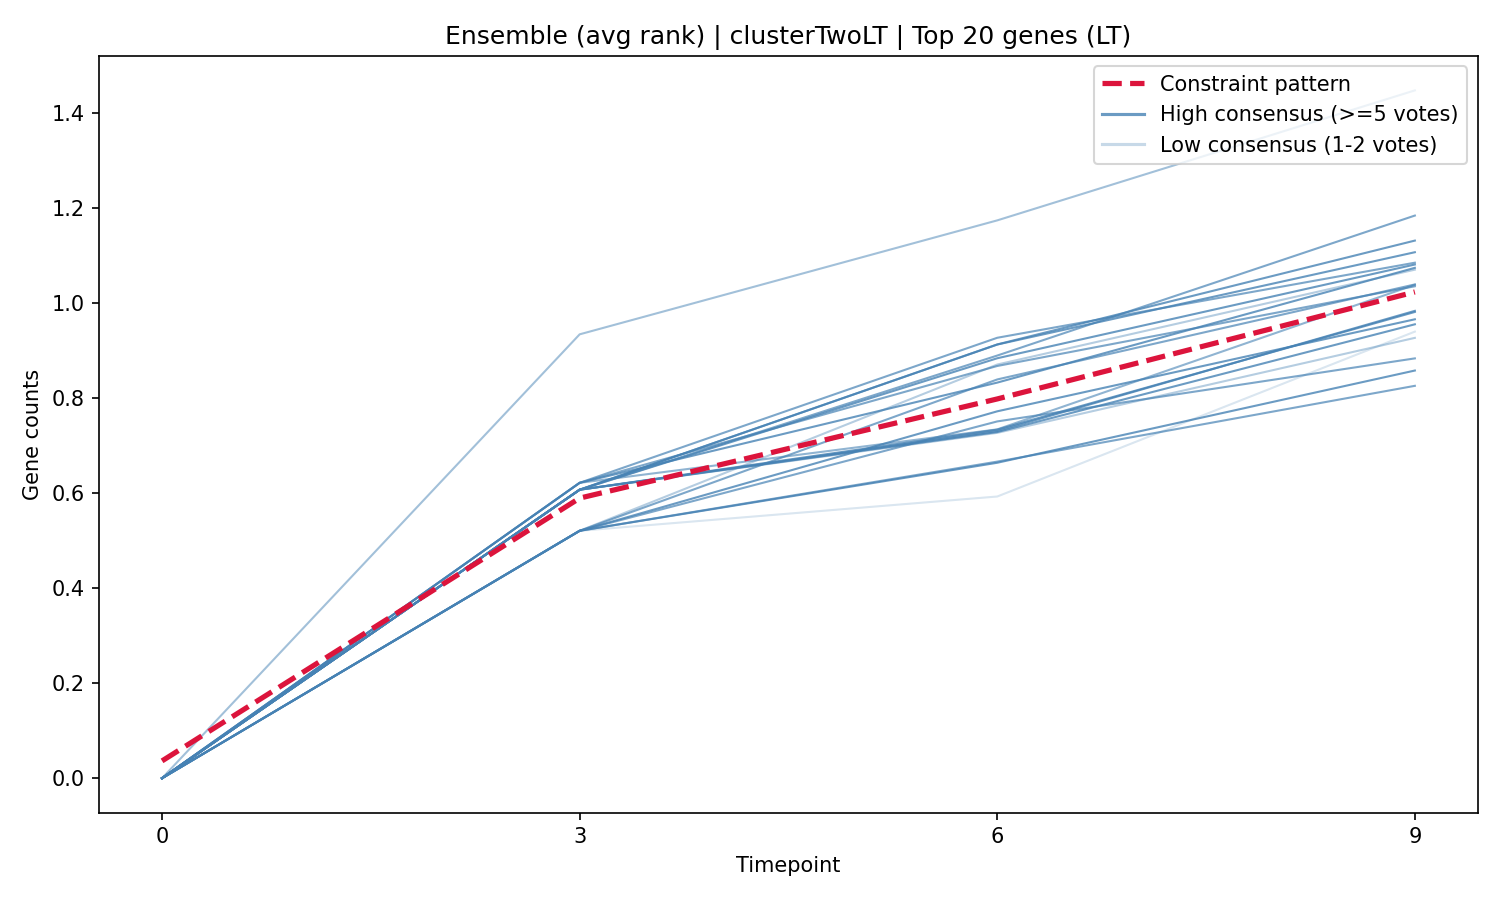
\includegraphics[height=0.85\textheight]{plots/Ensemble_LT_clusterTwoLT_constraint.png}
\end{frame}

\begin{frame}{clusterTwo LT — Overlap Heatmap}
\centering
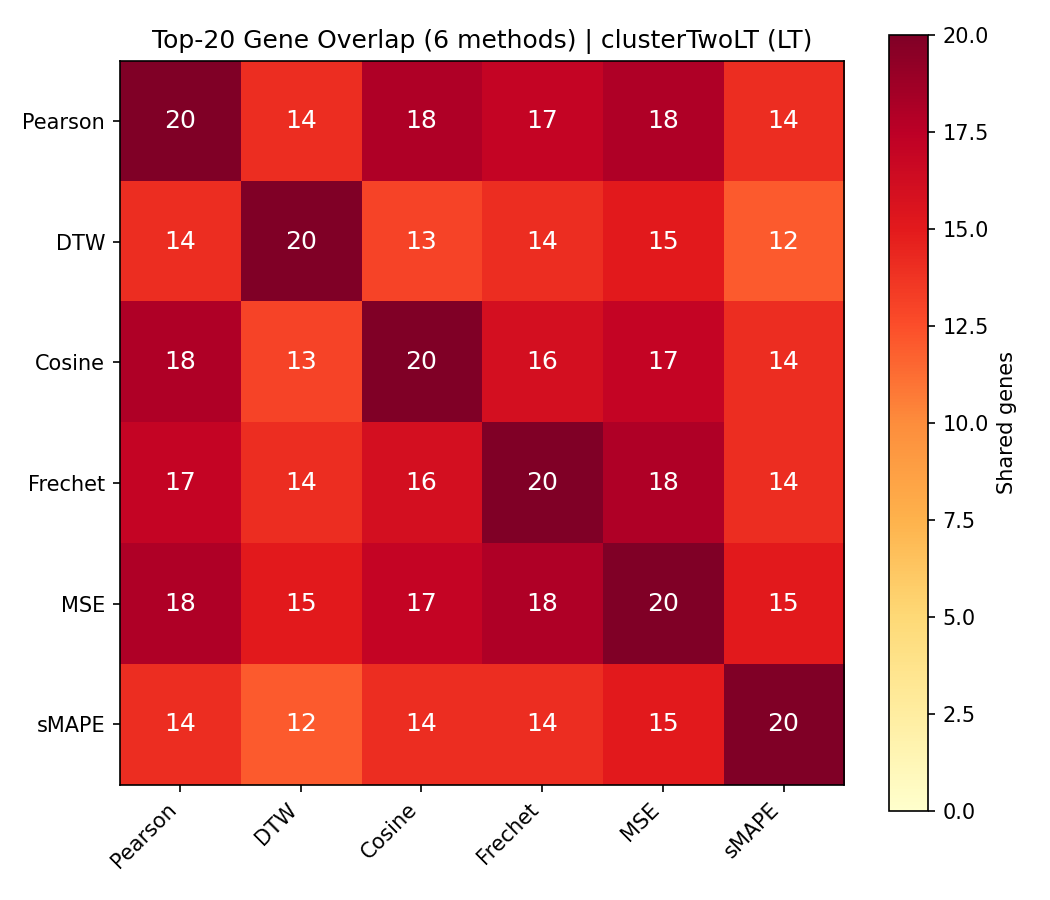
\includegraphics[height=0.85\textheight]{plots/overlap_6methods_LT_clusterTwoLT.png}
\end{frame}

% --- clusterThree LT ---
\begin{frame}{clusterThree LT — Pearson}
\centering
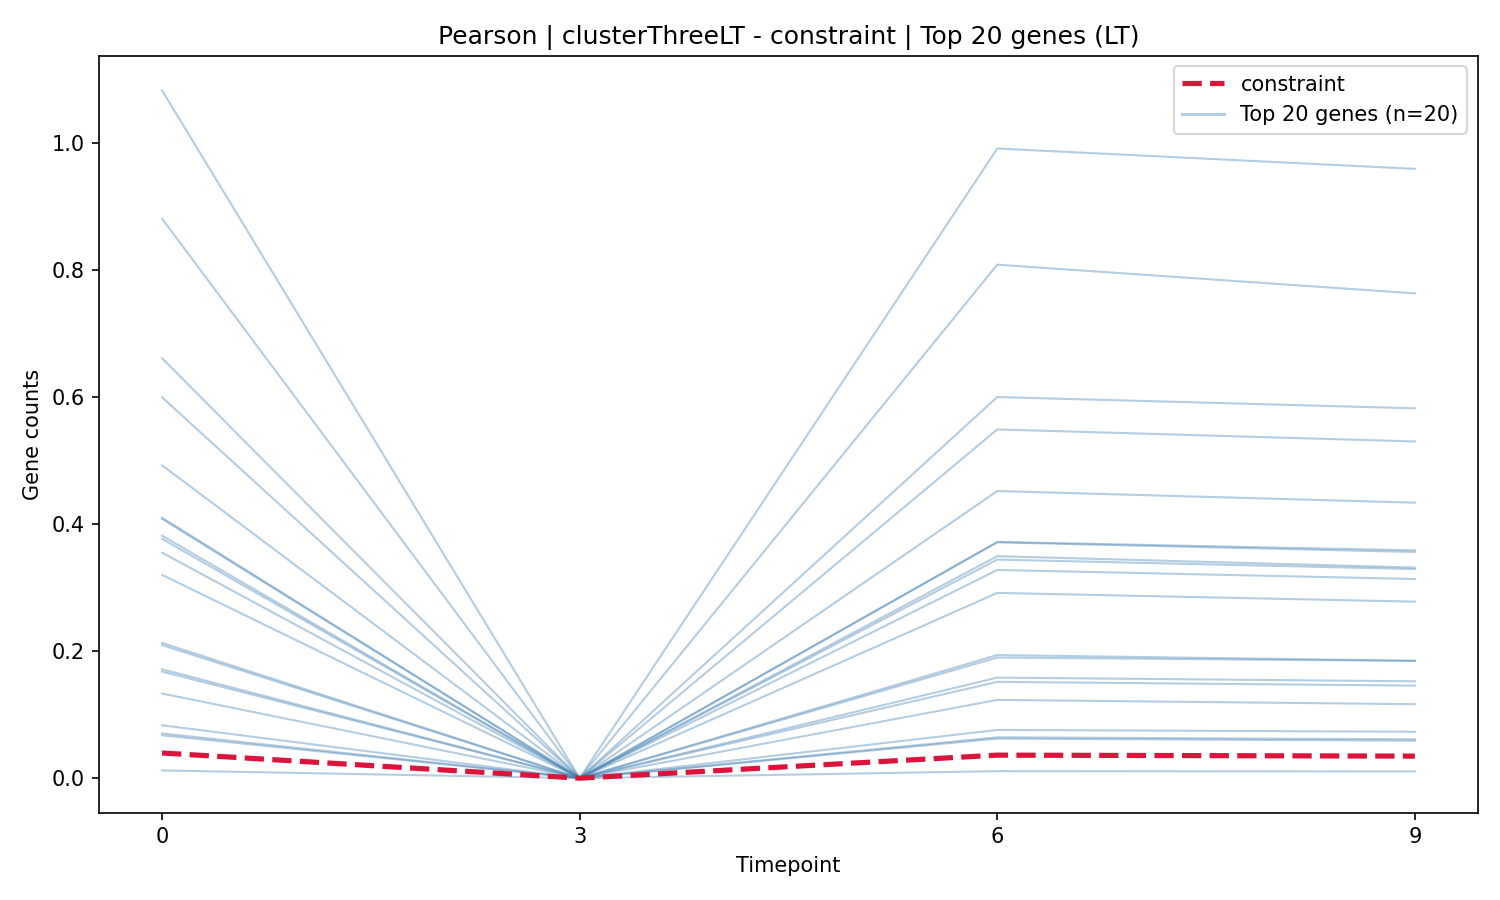
\includegraphics[height=0.85\textheight]{plots/Pearson_LT_clusterThreeLT_constraint.png}
\end{frame}

\begin{frame}{clusterThree LT — DTW}
\centering
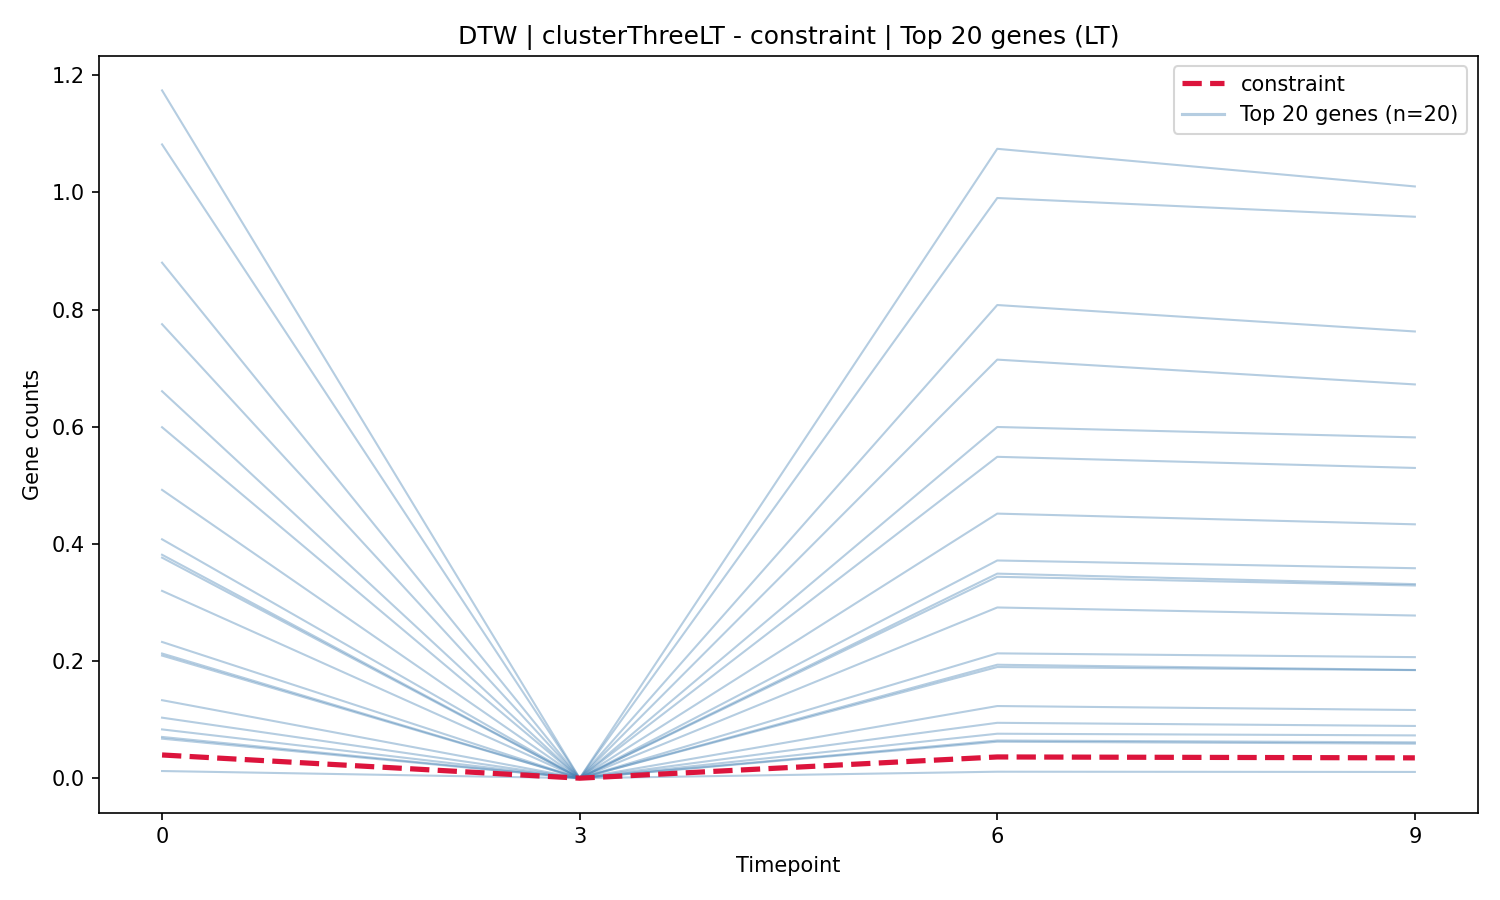
\includegraphics[height=0.85\textheight]{plots/DTW_LT_clusterThreeLT_constraint.png}
\end{frame}

\begin{frame}{clusterThree LT — Cosine}
\centering
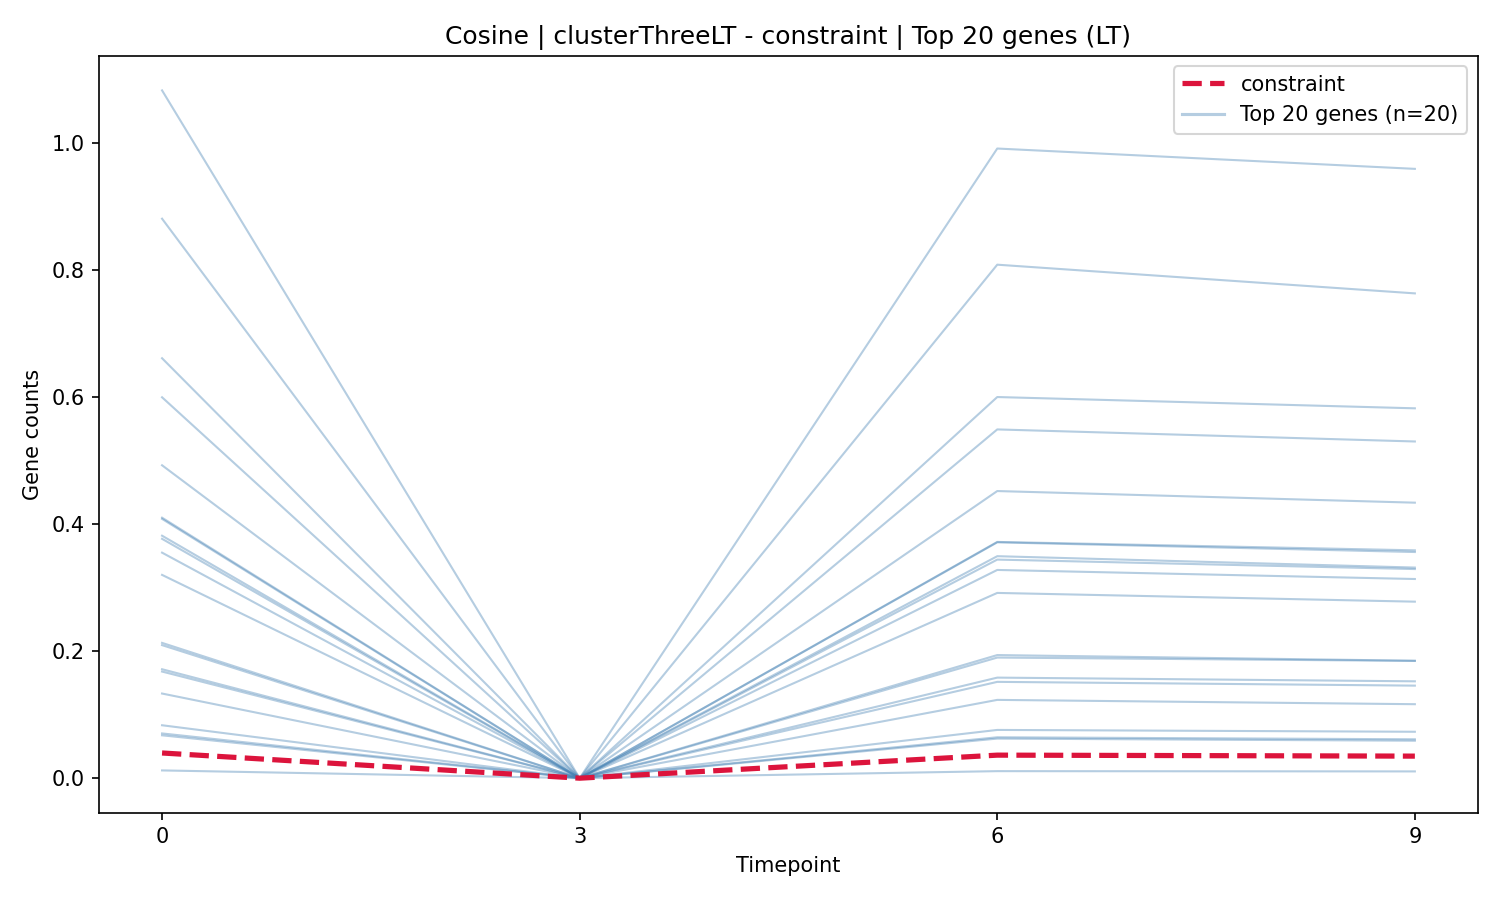
\includegraphics[height=0.85\textheight]{plots/Cosine_LT_clusterThreeLT_constraint.png}
\end{frame}

\begin{frame}{clusterThree LT — Fr\'{e}chet}
\centering
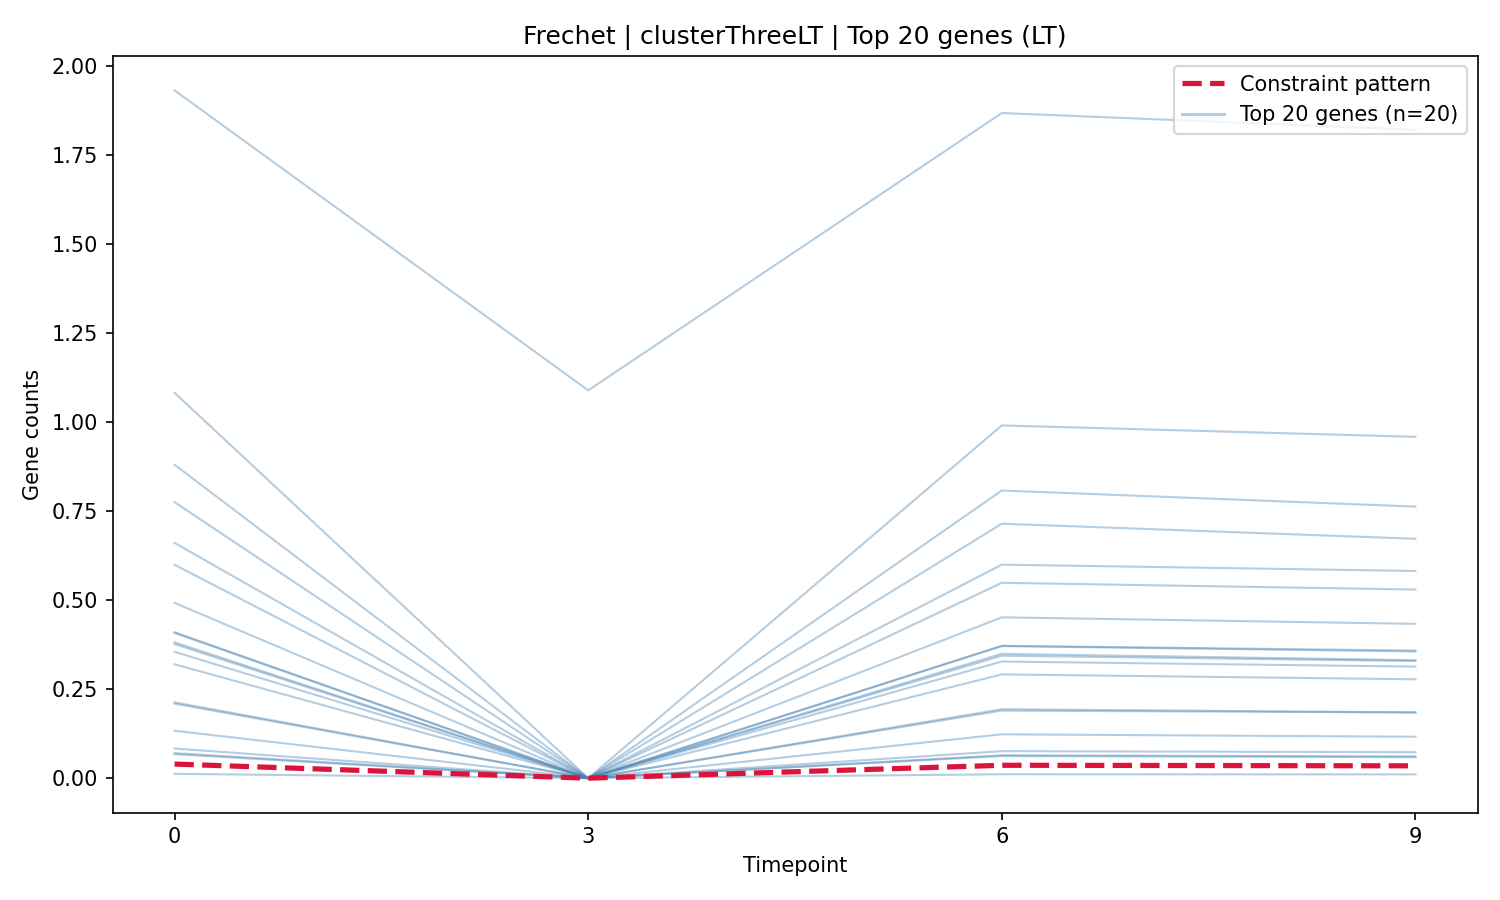
\includegraphics[height=0.85\textheight]{plots/Frechet_LT_clusterThreeLT_constraint.png}
\end{frame}

\begin{frame}{clusterThree LT — MSE}
\centering
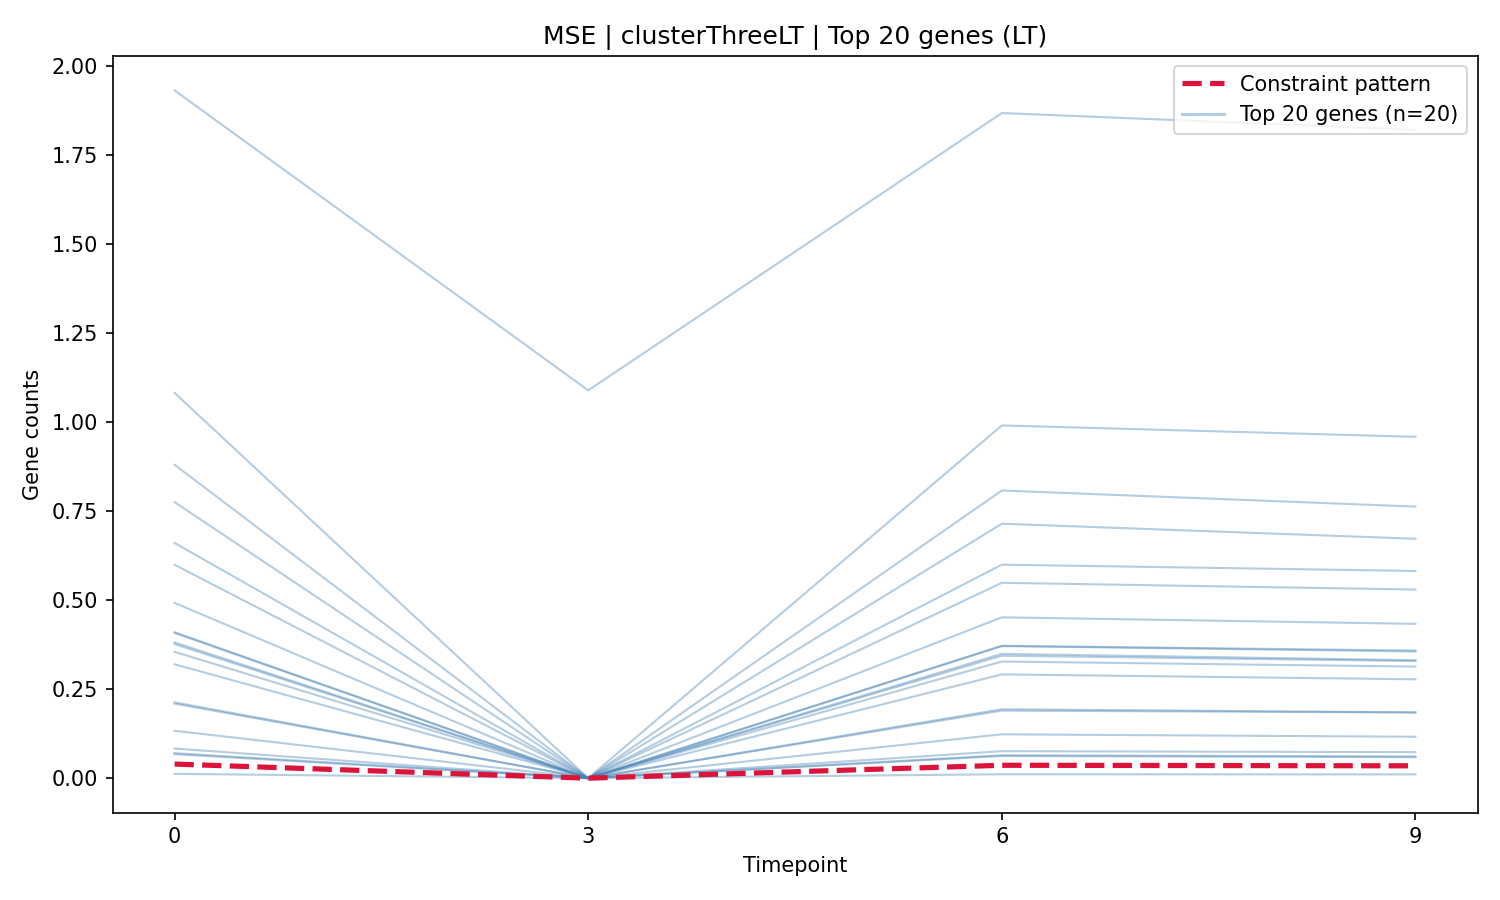
\includegraphics[height=0.85\textheight]{plots/MSE_LT_clusterThreeLT_constraint.png}
\end{frame}

\begin{frame}{clusterThree LT — sMAPE}
\centering
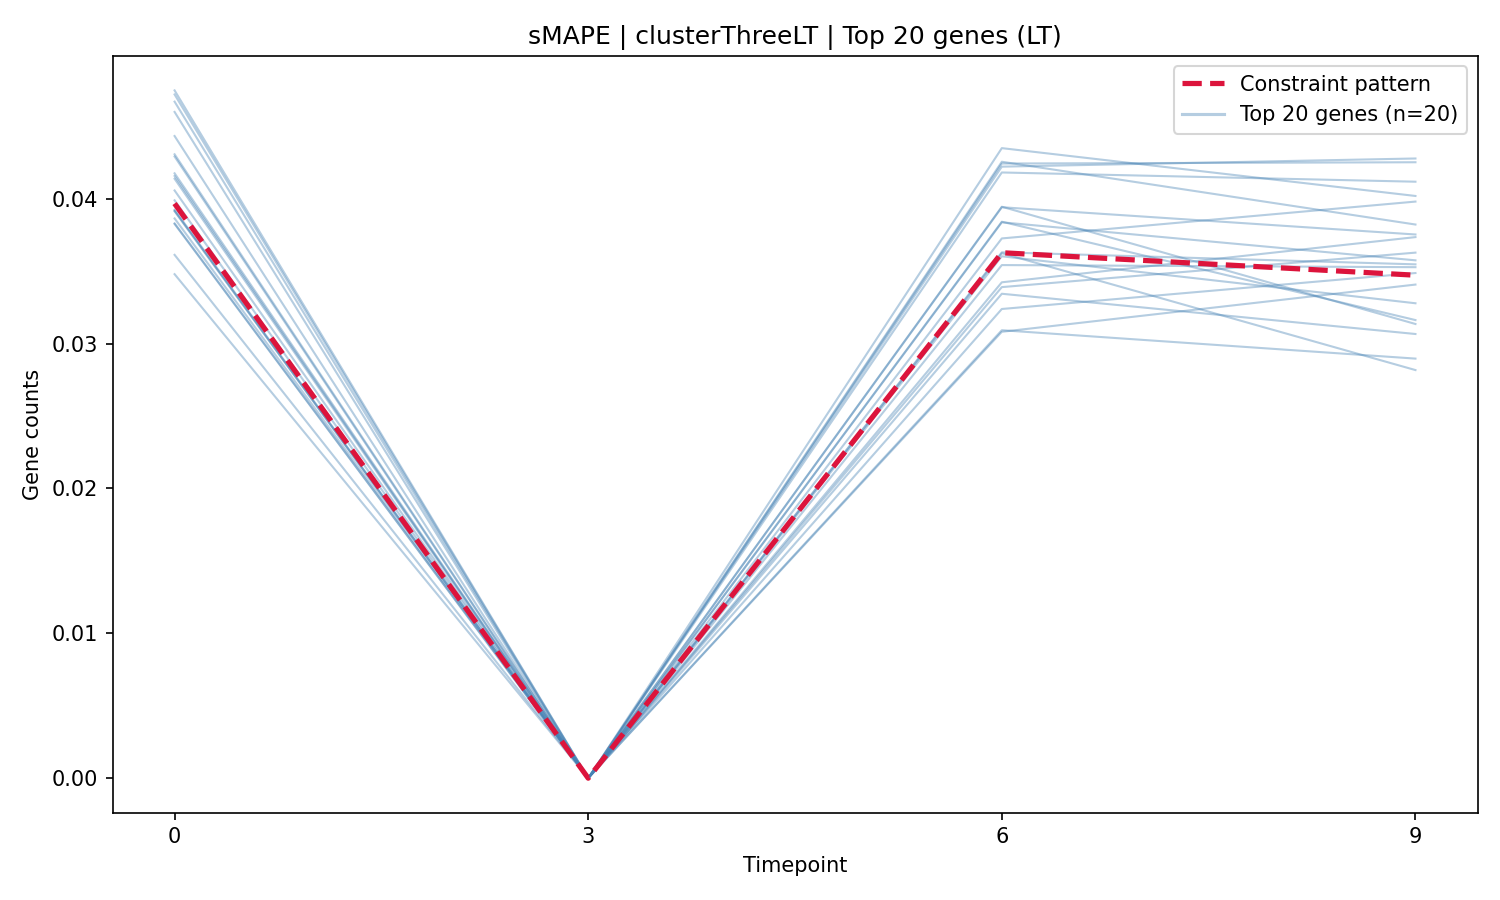
\includegraphics[height=0.85\textheight]{plots/sMAPE_LT_clusterThreeLT_constraint.png}
\end{frame}

\begin{frame}{clusterThree LT — Ensemble}
\centering
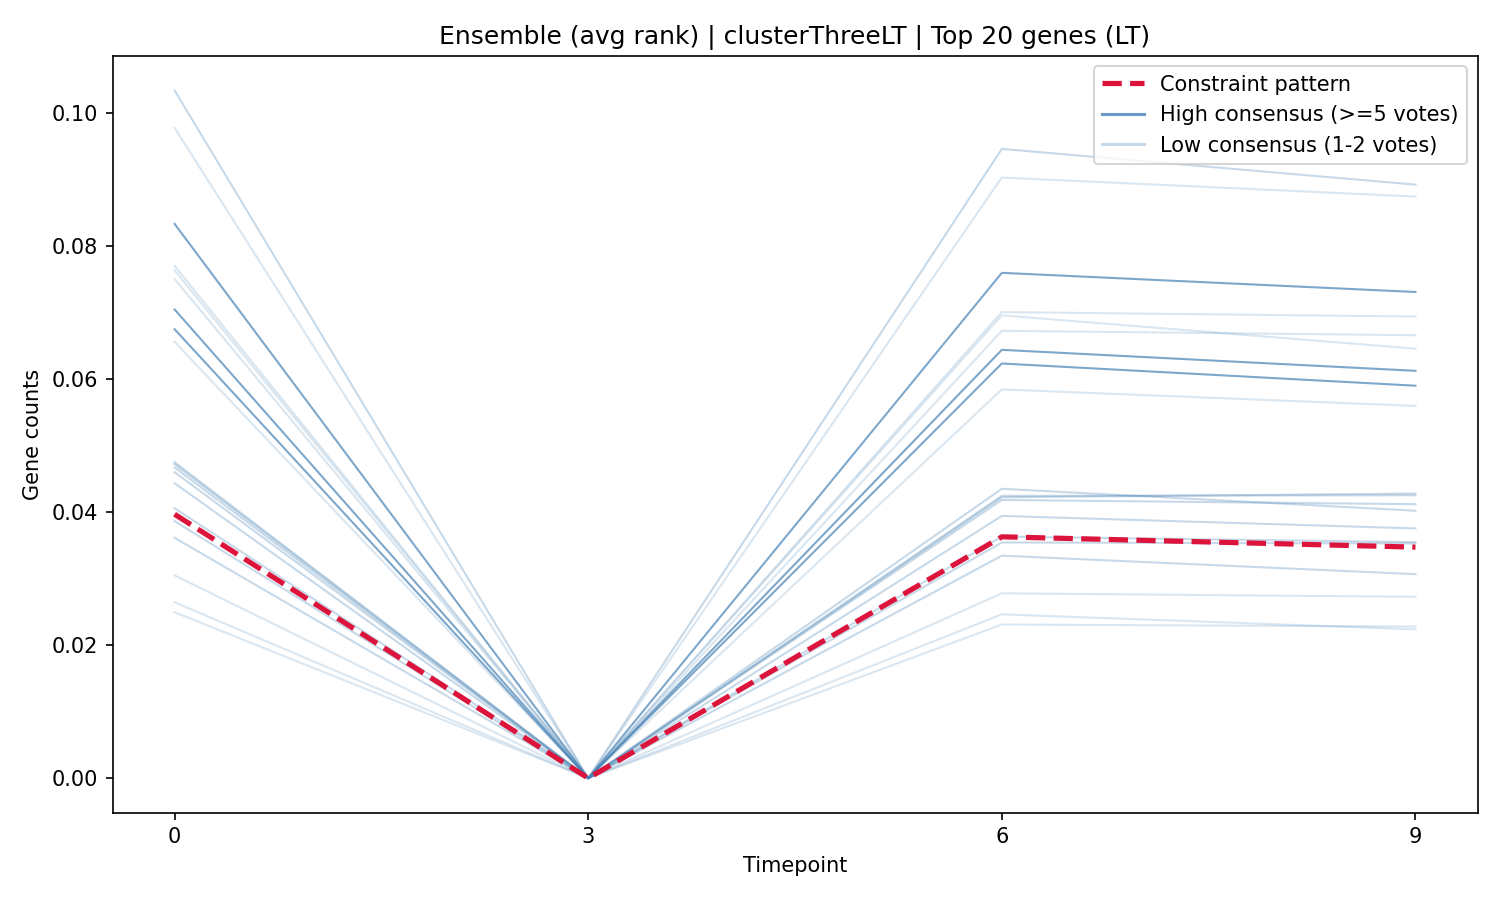
\includegraphics[height=0.85\textheight]{plots/Ensemble_LT_clusterThreeLT_constraint.png}
\end{frame}

\begin{frame}{clusterThree LT — Overlap Heatmap}
\centering
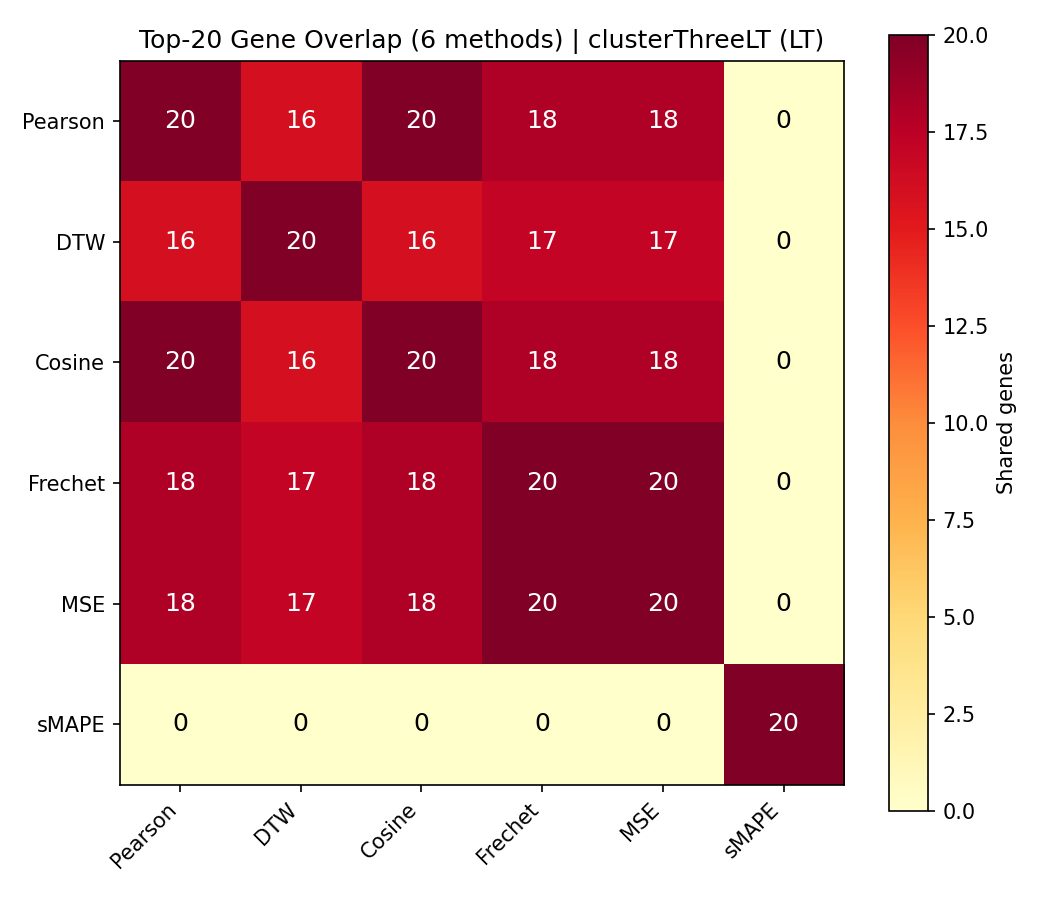
\includegraphics[height=0.85\textheight]{plots/overlap_6methods_LT_clusterThreeLT.png}
\end{frame}

% --- clusterFour LT ---
\begin{frame}{clusterFour LT — Pearson}
\centering
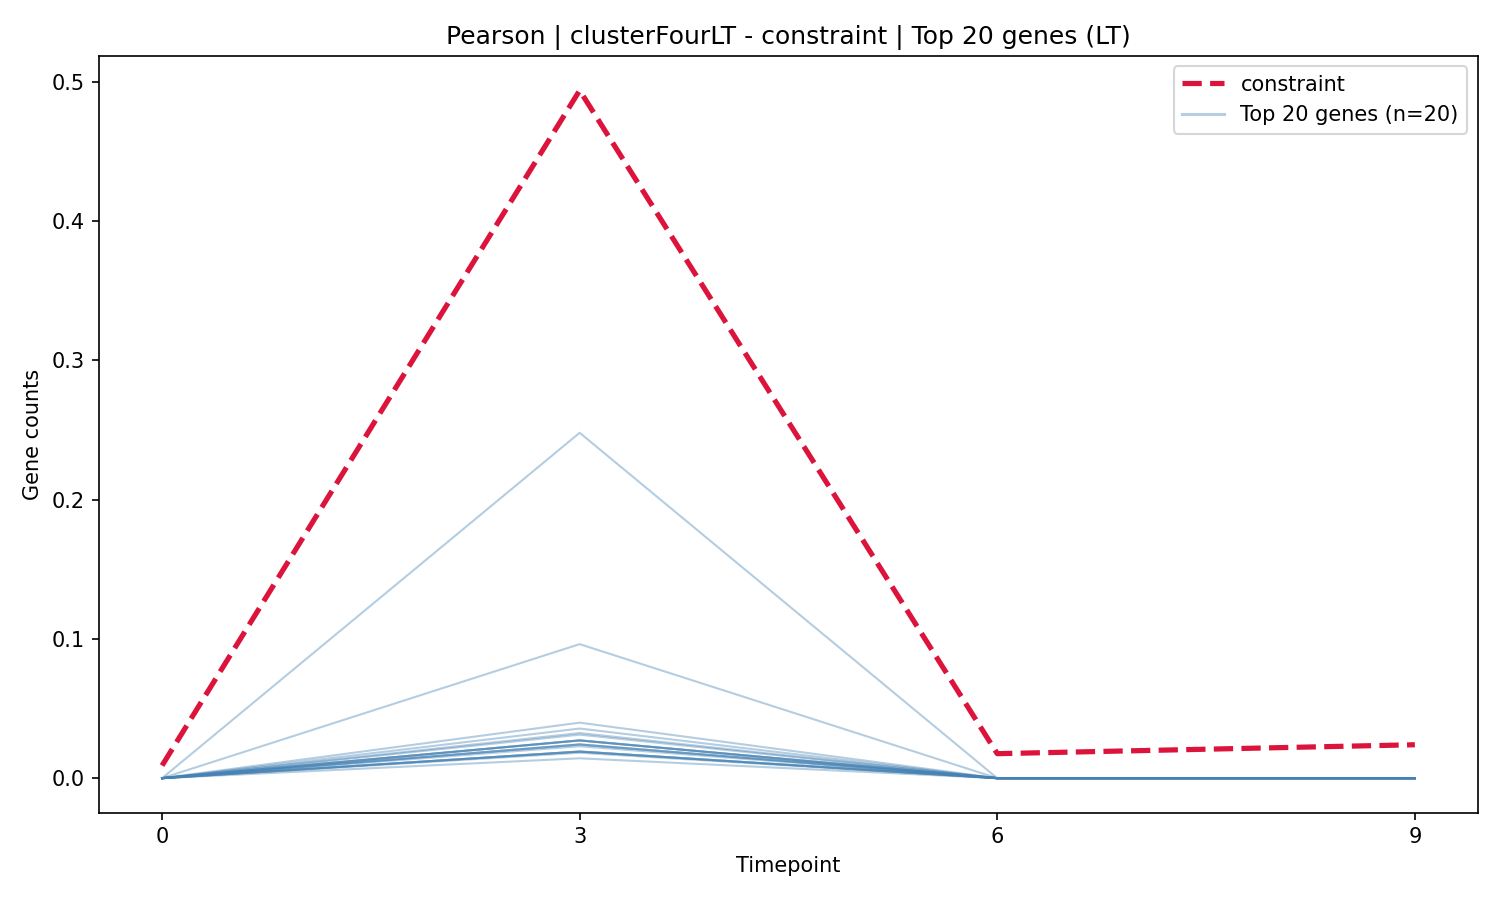
\includegraphics[height=0.85\textheight]{plots/Pearson_LT_clusterFourLT_constraint.png}
\end{frame}

\begin{frame}{clusterFour LT — DTW}
\centering
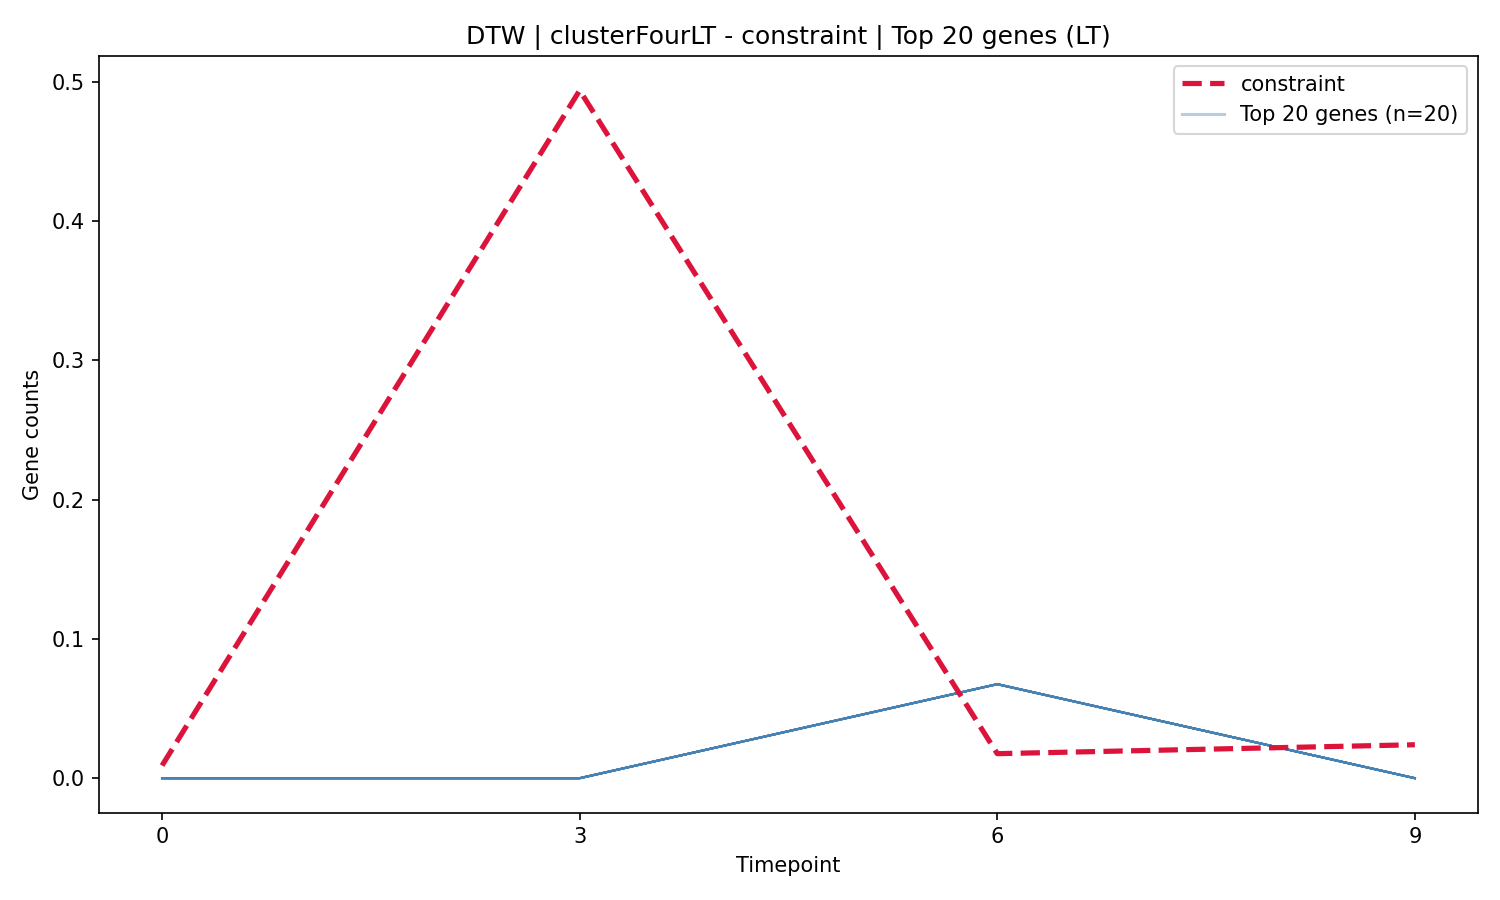
\includegraphics[height=0.85\textheight]{plots/DTW_LT_clusterFourLT_constraint.png}
\end{frame}

\begin{frame}{clusterFour LT — Cosine}
\centering
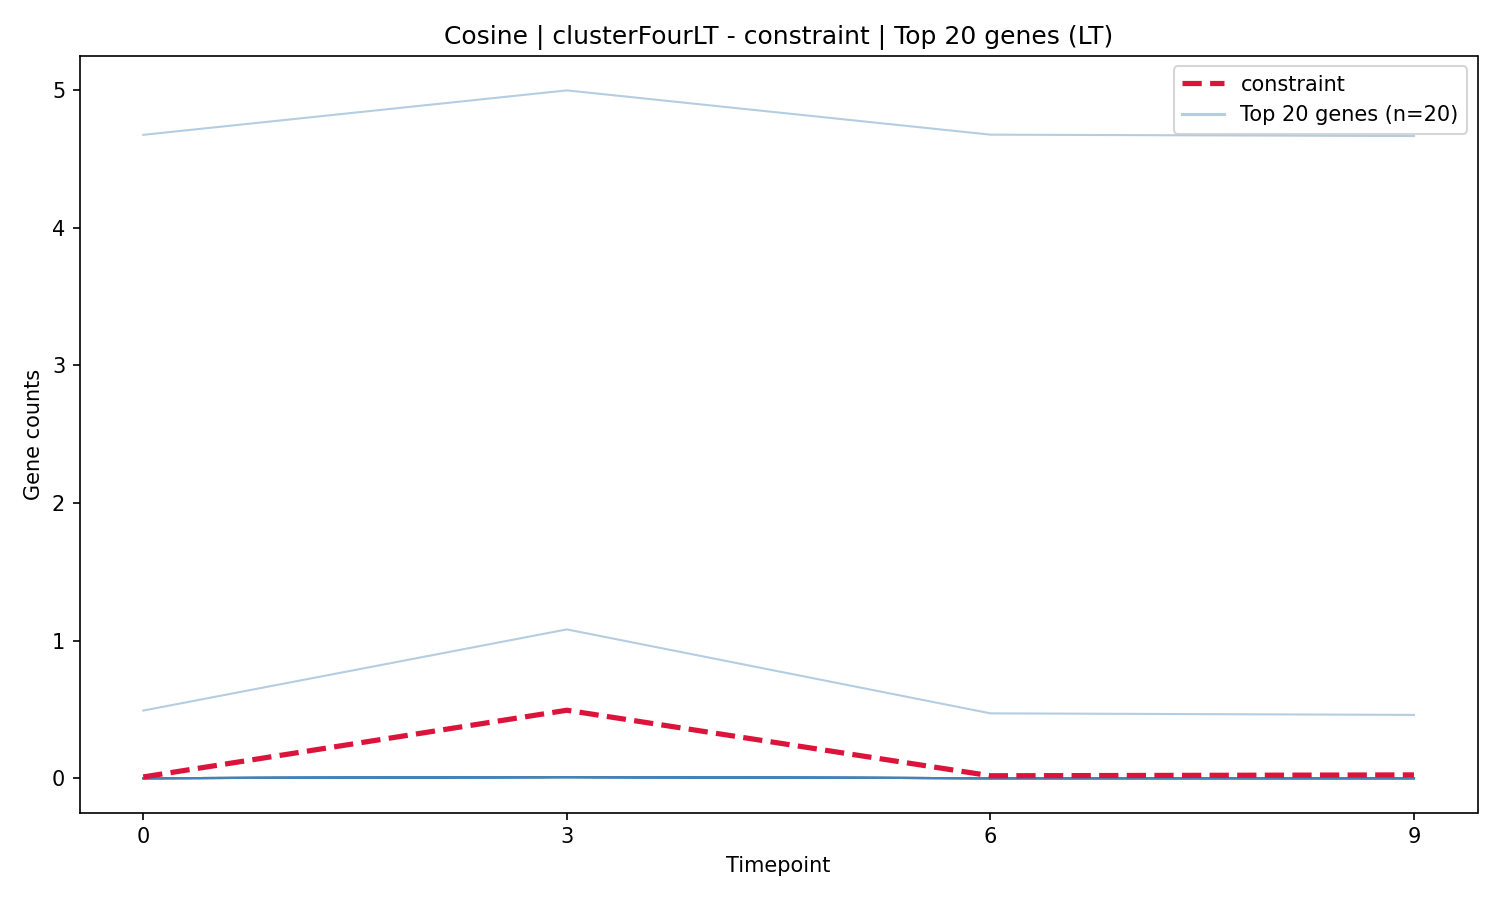
\includegraphics[height=0.85\textheight]{plots/Cosine_LT_clusterFourLT_constraint.png}
\end{frame}

\begin{frame}{clusterFour LT — Fr\'{e}chet}
\centering
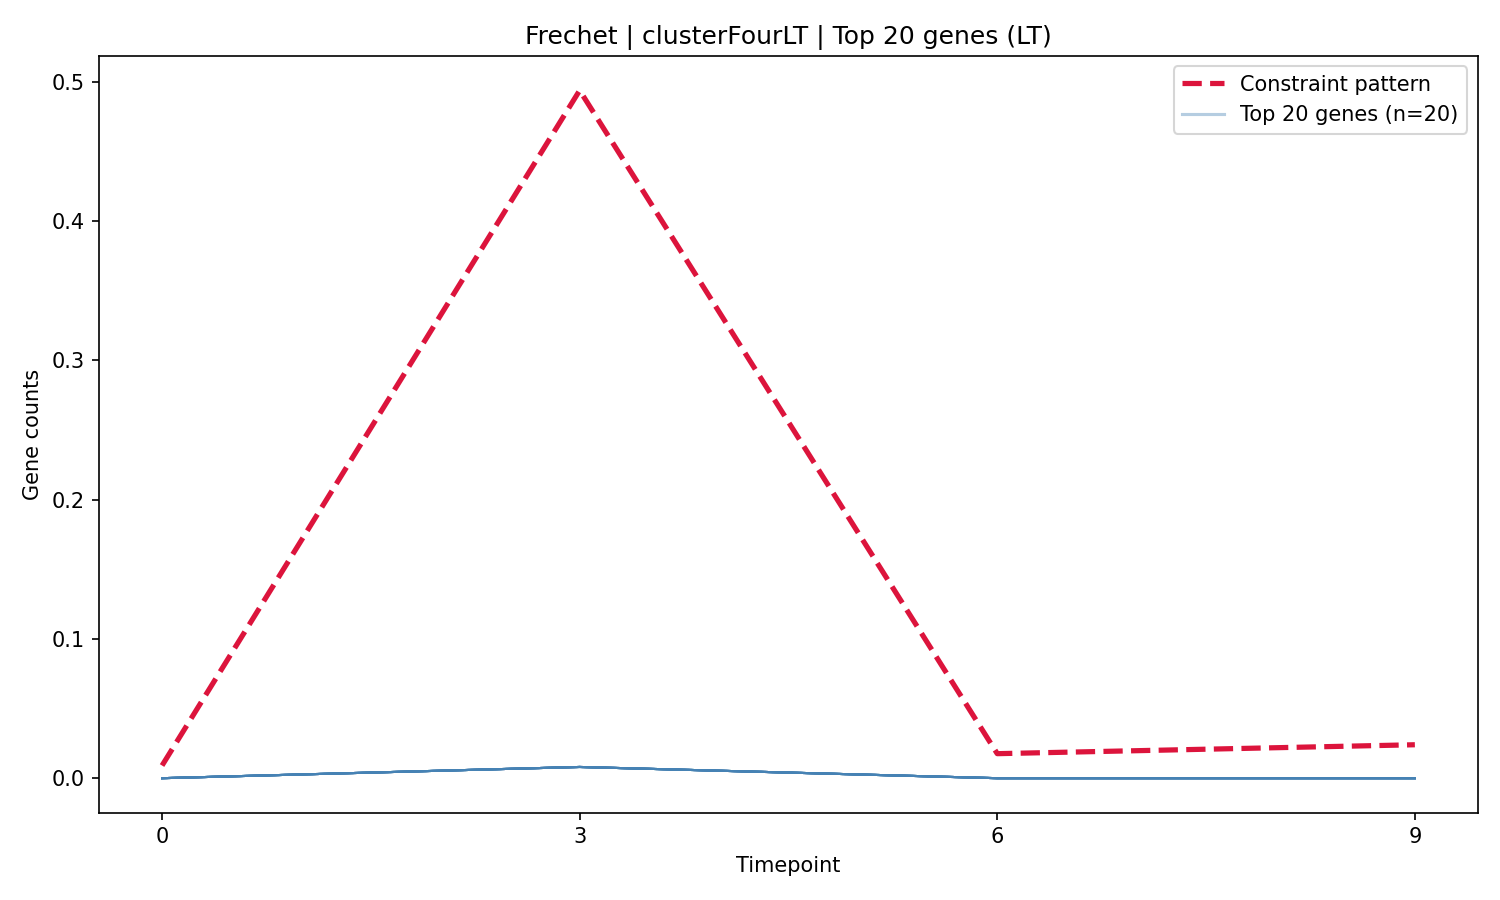
\includegraphics[height=0.85\textheight]{plots/Frechet_LT_clusterFourLT_constraint.png}
\end{frame}

\begin{frame}{clusterFour LT — MSE}
\centering
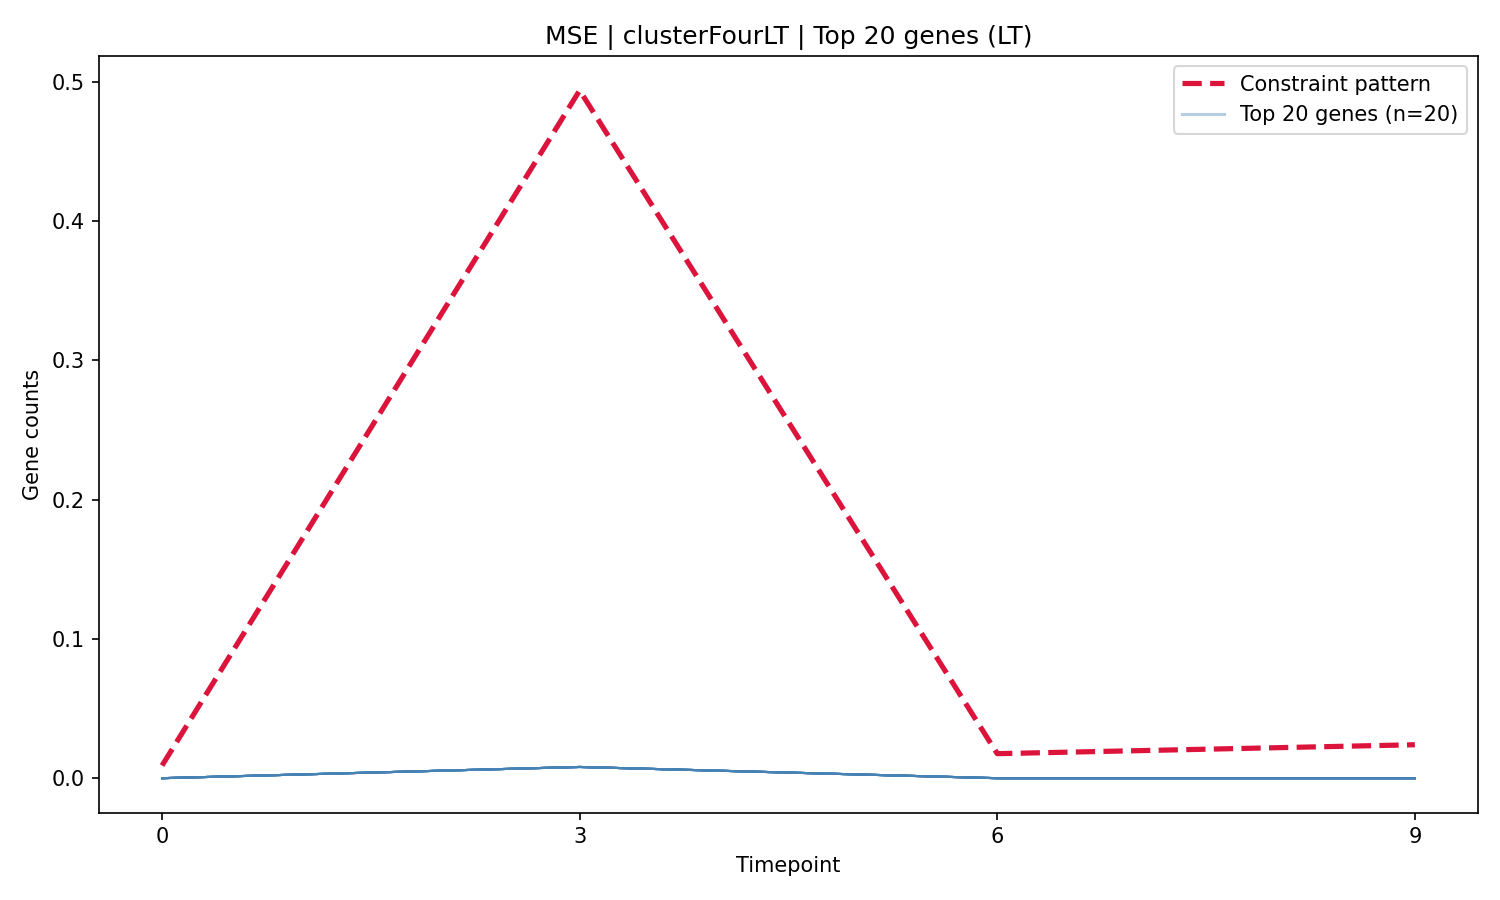
\includegraphics[height=0.85\textheight]{plots/MSE_LT_clusterFourLT_constraint.png}
\end{frame}

\begin{frame}{clusterFour LT — sMAPE}
\centering
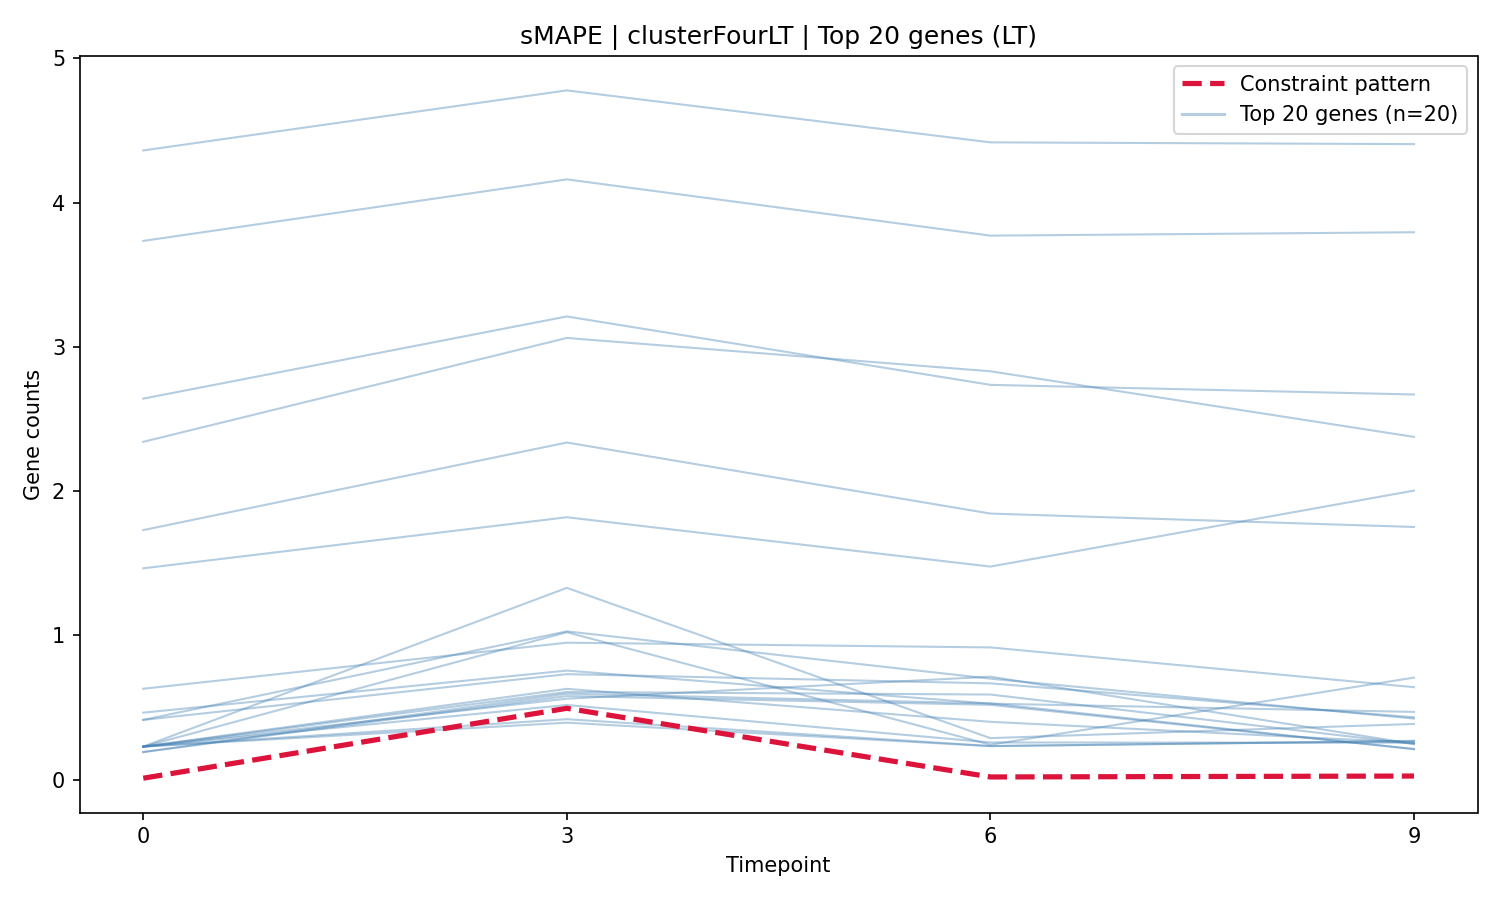
\includegraphics[height=0.85\textheight]{plots/sMAPE_LT_clusterFourLT_constraint.png}
\end{frame}

\begin{frame}{clusterFour LT — Ensemble}
\centering
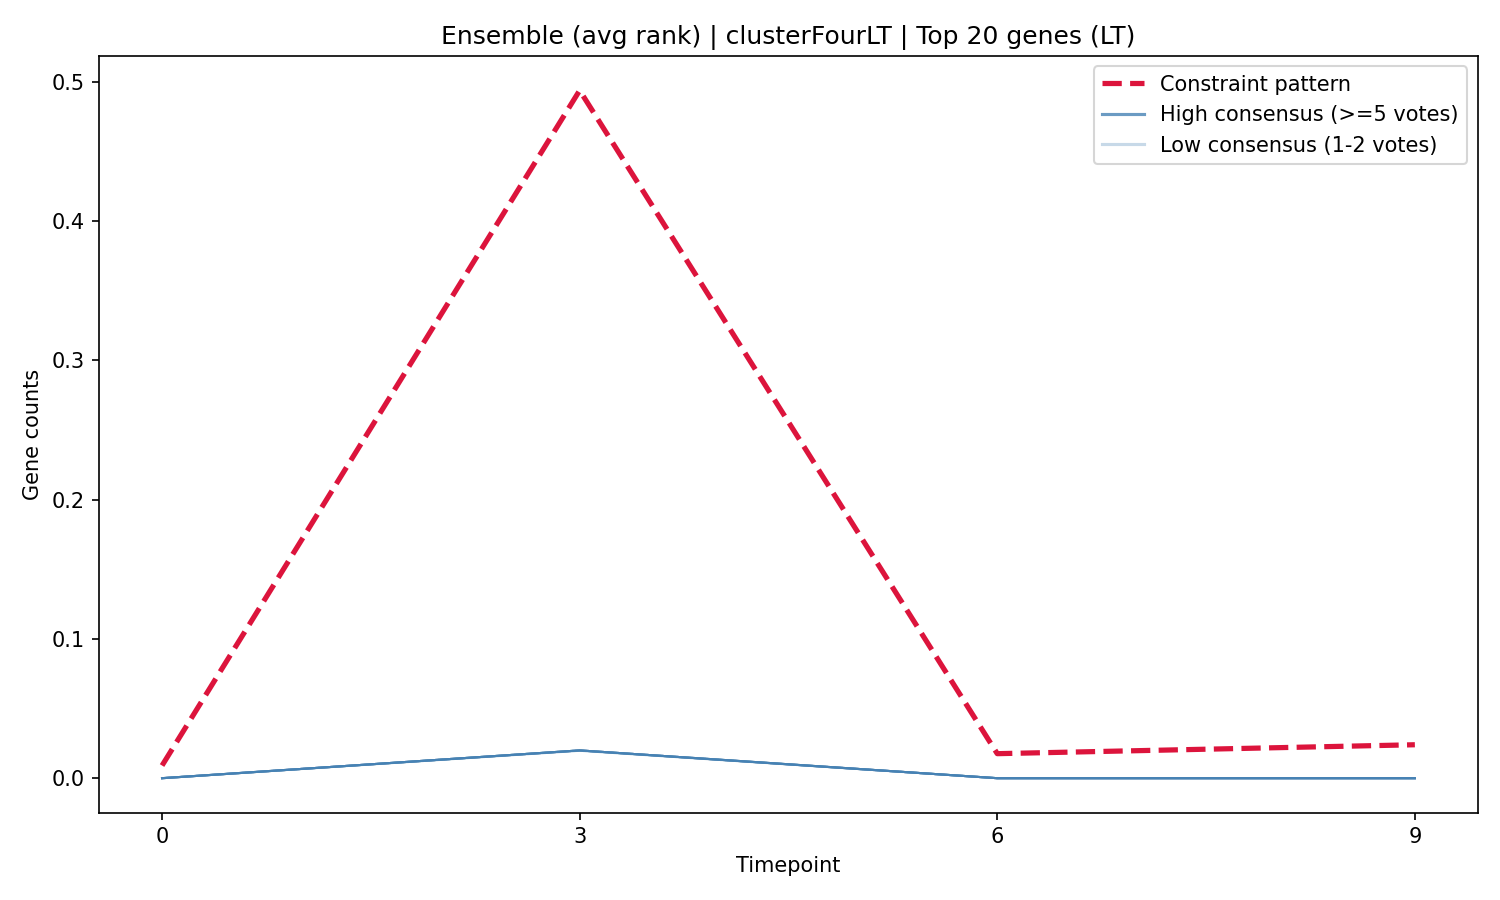
\includegraphics[height=0.85\textheight]{plots/Ensemble_LT_clusterFourLT_constraint.png}
\end{frame}

\begin{frame}{clusterFour LT — Overlap Heatmap}
\centering
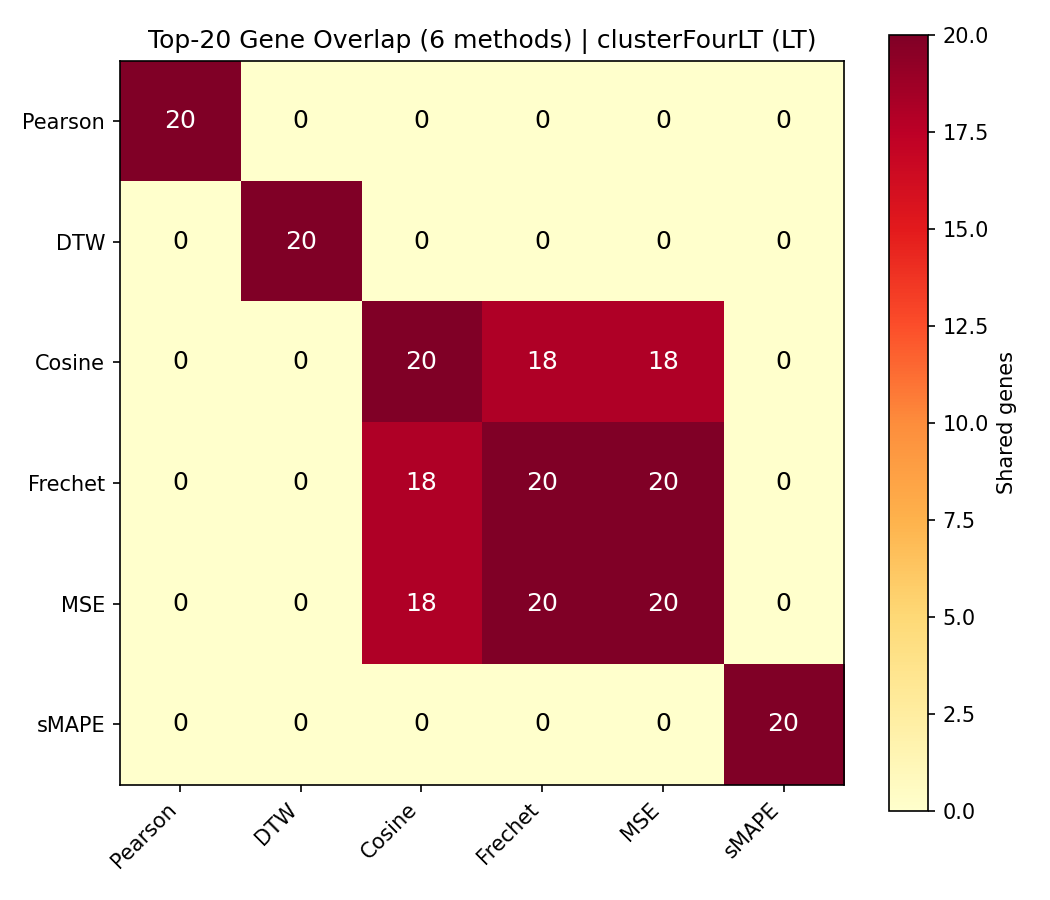
\includegraphics[height=0.85\textheight]{plots/overlap_6methods_LT_clusterFourLT.png}
\end{frame}

\end{document}
